% todo
% - url dazutun wo man dieses dokument runterladen kann & source usw
% - check all headings for proper capital writing
% - check all footnotes for being existent and unify them
% - oxygen icon theme lizenz

\documentclass[a4paper,10pt]{article}
\usepackage[utf8]{inputenc}
\usepackage{minted}

\usepackage{graphicx}

\usepackage{templates}
\usepackage{wrapfig}
%Das Paket erzeugt ein anklickbares Verzeichnis in der PDF-Datei.
\usepackage{hyperref}

\usepackage [left=2cm, right=2cm, top=2cm, bottom=2cm]{geometry}

% url package for clickable url files
\usepackage{url}

%Einrueckung eines neuen Absatzes
\setlength{\parindent}{0em}

\title{Multi-Platform Software Package Management}
\author{Joachim Schiele}
\date{2010-09-27 - 2011-03-26}

\pdfinfo{
  /Title    (Multi-Platform Software Package Management)
  /Author   (Joachim Schiele)
  /Creator  (c)
  /Producer (d)
  /Subject  (e)
  /Keywords (f)
}

\begin{document}



\begin{titlepage}
	\begin{center}
		%{\LARGE Eberhard Karls Universitt Tbingen}\\
		\includegraphics[height=3cm]{images/logo-uni-tuebingen.pdf}\\
		{\large			Fakult\"at f\"ur Informations- und Kognitionswissenschaften\\
								Wilhelm-Schickard-Institut f\"ur Informatik\\[2cm]}
		{\large 		Diplomarbeit Informatik\\[0.2cm]}
		{\LARGE\bf	Multi-Platform Software Package Management \\[1.5cm]}
		{\large 		Joachim Schiele  }\\[0.5cm]
								26. M\"arz 2011\\[2.5cm]
		\begin{center}
			{\small\bf			Erstgutachter \& Betreuer}\\[0.5cm]
			{\large					Prof. Dr. Herbert Klaeren}\\[0.2cm]
			{\footnotesize	Wilhelm-Schickard-Institut f\"ur Informatik\\
											Universit\"at T\"ubingen}\\[1.5cm]
		\end{center}
		\begin{center}

\vfill

This document and all the used pictures are available under the \\ \textbf{Creative Commons Attribution-ShareAlike License}\\

		\includegraphics[height=0.5cm]{images/cc.png}

For details see:

\url{http://creativecommons.org/licenses/by-sa/3.0/}

		\end{center}
	\end{center}
\end{titlepage}
\newpage
\tableofcontents
\newpage

\newpage
\section*{Abstract}
Today's package management is a complex field. This diploma thesis analyses different package management systems in several regards: how the packaging is done; how the user interacts with the package manager; Apt (Debian Linux), Portage (Gentoo Linux) and Nix (Nix OS) are compared in great detail. 

To get practical results, the author used the evopedia application, an open source offline Wikipedia reader, to experiment with several different package managers. This diploma thesis also tries to answer why there are no complex package managers for Microsoft Windows. Most package managers use their own terms which can not be generalized to other package managers. This problem was solved by defining meaningful words which describe certain properties of a package manager.  

\newpage
\section{Motivation}
\label{motivation}
Maintaining a package for several distributions requires lots of redundant work steps of its maintainers. This is because nearly all Linux distributions have their own unique package manager. Therefore one has to integrate (package) the software into each system separately. That is also true for distributions other than 'Linux distributions', still the situation is a bit different. \\

This is due to the fact that, often:
\begin{enumerate}
\item Software engineers are not 'also' doing deployment for their own software.
\item Software is developed mainly for one distribution.
\item Package management is not used while development but only when the software should be distributed.
\item Software development and package management (distribution) do not form a symbiosis.
\item There are problems in communication between users:
\begin{itemize}
\item Downstream and upstream: downstream patches are often not recognized by upstream.
\item Assignment of distribution specific bugs and upstream bugs are complicated.
\end{itemize}
\item Users / developers tend to bypass package management for convenience and therefore rely on a build systems to manage their dependencies instead of using the capabilities provided by the package manager.
\item Linux package managers mainly provide only one permission level which allows only one user or a group of users doing everything. Packaging can not be used by unprivileged users outside that group. The result, which was already mentioned, is that normal users tend to not use a package manager and therefore install/develop software bypassing it.

\item Users can't simply create their own packages and install them although most of the time they are allowed to build software from source and execute it.

\end{enumerate}

As we'll see, there have already been many attempts implementing different package management systems for various reaons. 
In the hope to help fixing some of the former mentioned issues and making packaging an easier task, I decided to investigate the state of the art of package management.

\section{Goal of this work}
The primary aspect of this thesis will be how software is integrated or can be integrated into distributions. As an example I decided to deploy the 'evopedia'\footnote{\url{http://evopedia.info/} - the offline Wikipedia reader} project, an offline Wikipedia reader, to a set of popular desktop distributions. While doing so I documented all the findings about different distributions and I'll discuss them in this thesis. However, as I'm using various Linux distributions and since I maintain several servers some additional findings were added.

One of my personal quests is to specify a multi-platform (or cross-platform) and a cross-distribution package manager which is capable of performing both source deployment and binary deployment. This seems as a natural step onwards, considering the advent of cross-platform software. \\

In short this thesis:
\begin{itemize}
\item Gives an overview about package management.
\item Specifies a multi-platform, cross-distribution package manager.
\item Lists features/shortcomings of package management systems.
\end{itemize}

This thesis introduces some new terms, as for instance: The 'sourceball'. Such definitions can be found in  \mbox{chapter \ref{Terminology}} and people not used to package management should start reading there. In this thesis I quote the Wikipedia which is normally a taboo to be used in scientific work. However, links to the Wikipedia have a very high link stability and most linked articles should be understood as a help to clarify terms/concepts used in this work. I also tried to explain concepts in detail for example by adding examples I tried to explain concepts in detail. 




\newpage
\section{Legal - License/Patent Issues}
\label{LicenseIssues}
This work clearly focuses on the technical side of 'Software Package Management'. But that does not mean that legal implications can be ignored.

Package management is used to share objects, like libraries, among several programs. That reduces duplicated work as the library needs to be written only once. Regarding the legal side, this also reduces the amount of code to be checked when certain program parts have to be verified using 'software verification'. However, the task on checking different licenses for compatibility is as complicated as picking the most appropriate license for a given software in the first place.

\begin{itemize}
 \item 'Open Source Software' (OSS) provides the necessary means to review security or stability\footnote{\url{http://www.dwheeler.com/secure-programs/Secure-Programs-HOWTO/open-source-security.html}} when having to rely on a third party product. This might not be that relevant for the 'big business', which has the ability to get source code for proprietary products anyway, but most likely, for all others.

 \item 'Free and Open Source Software' (FOSS/FOSS)\footnote{\url{http://en.wikipedia.org/wiki/Free_and_open_source_software}} has an even stricter set of rules on what legal obligation are applied to each side. However, it depends on the strategy on how to position a product on the market and might vary from situation to situation. 

 \item When doing 'Package Management' it is very important to know the legal state of the used toolchains. Examples:
\begin{itemize}
 \item 'C/C++/Objective-C', Mac OS X: \\Requires the user to install Xcode manually, prior usage, as Xcode is restricted for not being redistributed. Automated downloads are forbidden (known as a 'fetch restriction'). This also implies that the Xcode installation is not subject of any package manager and requires manual deinstallation. \\Note: Toolchains with such restrictions are referred to as 'impure' in Nix terms.
 \item 'Java', Gentoo Linux: \\Java (Oracle) is restricted not to be redistributed and also enforces a manual download ('fetch restriction') though some distributions, such as Gentoo, for example, provide wrapper scripts to install it via Portage so that both JRE and JDK are covered by package management (in contrast to Xcode where this is not the case).
 \item '.NET and C\#', Windows (Micosoft):\\ Altough there exists a free implementation called 'Mono' it is not a full replacement yet. And even when one assumes 'Mono' could be used as a drop in replacement for '.NET', there are still patent issues\footnote{\url{http://www.fsf.org/news/dont-depend-on-mono}} to be expected.
\end{itemize}

\end{itemize}

\subsection{Import/Export and Usage}
This is actually one of the most challenging parts of package management, both for commercial and free package managers as: 
\begin{itemize}
\item \textbf{Exporting} certain software might be illegal in some countries. The export of 'cryptographic software' was forbidden in the USA\footnote{\url{http://en.wikipedia.org/wiki/Export_of_cryptography_in_the_United_States\#US_export_rules}} for a very long time.

\item Also \textbf{importing} can be illegal, as stated by rsa.com\footnote{\url{http://www.rsa.com/rsalabs/node.asp?id=2333}, Title: What are the cryptographic policies of some countries?}.

\item Not to forget \textbf{sanctions}\footnote{\url{http://sourceforge.net/blog/some-good-news-sourceforge-removes-blanket-blocking/}} against imports/exports.
\end{itemize}

\subsection{Software Patents}
By far the biggest problem is that 'Software Patents' are handled differently in each country. This thesis will not cover if software patents are good or bad. To avoid being sued because of distributing software which is obviously affected by 'Software Patent' claims, some downstreams\footnote{\url{http://en.opensuse.org/Restricted_formats}} simply do not distribute such software. There has been no official support for MP3 and certain video codecs in popular distributions as SuSE Linux (at least after being sold to Novell). This is also true for Fedora and most others.

To support such questionable code at all, many downstreams support (directly or indirectly) 'third party' software repositories.

\subsection{Richard Stallman (GPL/LGPL/AGPL)}
Although open source licenses as the BSD license existed long before the GPL, LGPL or AGPL, it seems that they fill a very important role for many developers nowadays. When comparing the GPL with the BSD license both are open source licenses and both are used often. The main difference is that the BSD license is too free and motivates non-free projects to use the codebase without giving anything back. The BSD licenses make strong vendor lock-in easily possible.

\subsection{Lawrence Lessig and the 'Creative Commons' (CC) License}
As software packages contain not only code and especially since the GPL-/BSD- or FDL-Licenses do not apply well to things other than code, a completely new set of licenses, the Creative Commons licenses, had to be created. One of the most prominent uses of the CC license is the Wikipedia project. This includes the articles (the database) but also the pictures, sounds, music and various other formats.

\subsection{Vendor Lock-In}
Open source basically preserves freedom to use software in various ways. It helps to review code changes and enforces upstream to create updates only when needed. Therefore it minimizes vendor lock-in and liberates 'Software Package Management' as it makes it possible in the first place.

In contrast, there is a relatively new development, most often referred to as something like an 'App store'. There are many popular implementations as:
\begin{enumerate}
 \item Apple's ``App Store`` for iOS and Mac OS X
 \item Valve's Steam platform for software/media distribution
 \item Sony's PS3 Console and the PS3 Network  /  Amazon Kindle and Orwell 1984
 \item SDKs for developers as Xcode, Java and .NET
\end{enumerate}

There are so many more similar platforms used to install software but they all have a few things in common. The most important aspect of each platform is the control of the distribution path and whenever possible also of the content being distributed. They seem to enforce their policies by all means necessary.

Before concepts like 'App stores' were common, software was usually installed from a floppy/CD/DVD. The operating system was designed to execute all kind of programs and the only limitations were GPU/CPU boundaries. This has changed very much lately. Apple bans\footnote{\url{http://www.golem.de/1101/80668.html} VLC wegen Entwicklerbeschwerde aus app store entfernt} GPL software from their 'App Store'. Many games require 'Steam' to be run as a dongle like service while the game is executed. More often than not, Steam also requires a working internet connection, even to execute games typically played offline. Many Steam powered games save game states online, using the 'Steam cloud'. When starting Steam it checks for updates and if one is found for an installed game, one cannot play the game online until the update is performed. Steam forces such updates even though others would also not want to update (say by using the same 'old' version). \\
Sony removed a fundamental feature called 'Other OS\footnote{\url{http://en.wikipedia.org/wiki/OtherOS}}'. This was done with a software update, which was required either to play newly bought games or when wanting to be part of the 'Playstation3 Network', which is required for online gaming. And finally there is the Amazon platform to distribute ebooks for the Amazon Kindle. Interestingly, the platform seems to be able to remove \footnote{\url{http://news.cnet.com/8301-13860_3-10289983-56.html}} virtually any 'book' from the device. Fun fact: they removed 'Orwell's 1984'.

To sum up, most of these platforms take a lot of the user's freedom. As already shown they can alter 'terms of use' any time forcing anyone to agree. They can remove features or software any given time. This is not even the worst case scenario. The important thing is to know this before relying on such distribution channels.

And finally some words about some popular SDKs: Apple's Xcode requires to have an 'Apple Developer ID' to be able to download the SDK itself. This makes 'source deployment' a very cumbersome experience for new users especially as many of the Xcode developer tools used with Homebrew or Nix are taken from the GNU toolchain which are open source tools. 

\begin{quote}
\textit{The Xcode suite includes a modified version of free software GNU Compiler Collection (GCC, apple-darwin9-gcc-4.2.1 as well as apple-darwin9-gcc-4.0.1, with the former being the default)}\footnote{\url{http://en.wikipedia.org/wiki/Xcode}}
\end{quote}

With this in mind, how is package management affected? Since the Xcode package, which containins the toolchain to build software, is non-free or consists of certain non-free components it makes complicated issues likely. 

\newpage
Possible Xcode issues:
\begin{enumerate}
 \item Xcode download has a 'fetch restriction'
 \item Redistribution of the same Xcode package (download url) but with different content \\
       (might not have happened to Xcode yet, but such things happen\footnote{\url{http://bugs.gentoo.org/67266} Gentoo Bugzilla Bug 67266})
 \item Manual installations/deinstallations/updates issues of Xcode
 \item The installation of Xcode bypasses package management
 \item Incomplete installations or broken updates
 \item Improper checksums of Xcode downloads (because of custom tagging\footnote{\url{http://www.google.de/search?sourceid=chrome&ie=UTF-8&q=Topic+:+Xcode+3.2.5+checksum}} with Developer ID)
 \item No guarantee for legacy download support of old Xcode versions combined with inability to redistribute Xcode
\end{enumerate}
Looking at this list of possible issues it should be clear that one will have a hard time to guarantee reproducibility with such a toolchain.

In contrast there are other 'App stores' which offer commercial and free software at the same time. Examples:
\begin{enumerate}
 \item Maemo 5\footnote{\url{http://maemo.org/downloads/product/Maemo5/evopedia/} Maemo 5 portal for the open source evopedia application} (Nokia) and the OVI store (for example used in the N900 smart phone, where one can add 'open source' projects without having to pay). This is the main platform for evopedia development in the year 2010.
 \item Probably most Linux based mobile platforms as the 'Android Market' (Google) used on Android.

\end{enumerate}

\subsection{Legal Problems When Distributing modified Programs in Binary Form} 
There are some licenses as the MPL (Mozilla Public License)\footnote{\url{http://www.mozilla.org/MPL/mpl-faq.html}} which forbid to distribute modified binaries, using the upstream project name. The Mozilla Corporation requested 2006, to rename Firefox to a different name, if the Debian Project wants to continue distributing binaries based on modified source code. Since then the Mozilla programs do have new names on on Debian Linux. Doing 'source deployment' this would not be an issue (for example using Gentoo Linux).

\subsection{Source Deployment vs Binary Deployment}
Binary Deployment requires redistribution of upstream related material. So all material has to be checked for proper licensing. That means a user of a distribution using 'binary deployment' downloads all software from downstream. In contrast there is 'source deployment' where all software is downloaded from upstream instead. Doing 'source deployment' the compilation process is not done on a remote machine but instead on the local computer. That implies that patching software is now in a different context which changes the legal situation.

For 'binary deployment' it is also important to trust downstream, as compiled software can not be verified to be unmodified as claimed by downstream. This implies that 'binary deployment' using binaries of downstream might not be appreciated by all users. The use of asymmetrical cryptography makes the situation better in some ways (signing files using GPG), however it only helps to reveal modifications which happen while packages get copied over a network by attackers. That means the guarantees are like in HTTPS, where not the contents itself but the distribution ways are secured.





\subsection{Summary}
Seen from the legal perspective, it seems to be a good idea to use a FOSS toolchain because of the 'free' nature which makes vendor lock-in much harder to enforce. This is important as it makes popular toolchains more persistent, thus reliable.

In the context of this thesis it should be noted that the most complex, and therefore more powerful package managers, exist where packages mainly consist of open source software. However, these package managers are capable of doing closed source deployment (as done with Skype) as well but show the full potential with open source mainly. 













\newpage
\section{Package Manager Analysis}
\label{PackageManagerAnalysis}
This chapter is about the definition what package management\footnote{\url{http://en.wikipedia.org/wiki/Package_management_system}} actually is. It contains a list of various features implemented in package management systems, which are briefly discussed. In chapter \ref{packagemanagementanalyzis} we are using that knowledge looking at today's package managers to find out what they have in common and where they differ, as for instance by implementing unique features.









\subsection{Components used in a Package Manager}
\label{ComponentsUsed}
Package management can be split into different modules which compose the package manager:

\begin{figure}[h]
\caption[Package management]{Different modules of a package manager}
  \centering
\label{fig:package_management}
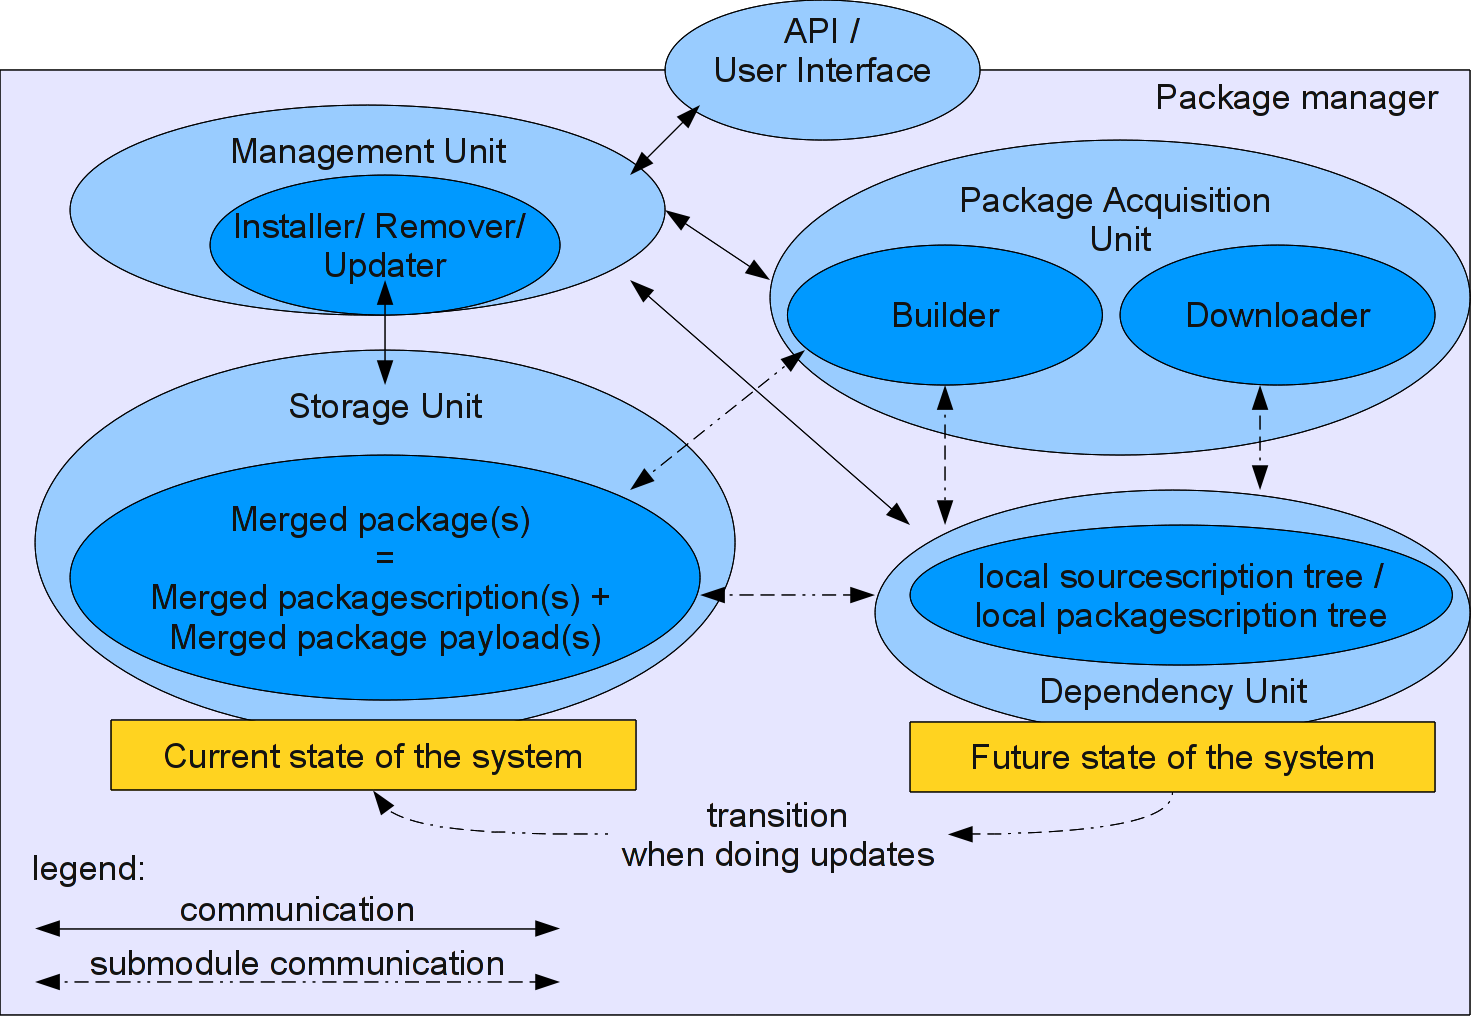
\includegraphics[width=120mm]{diagrams/package_management.png}
\end{figure}

\begin{enumerate}
\item \textbf{API/User Interface}\\
Expose the functionality of the package manager to the outside world by providing an API external tools can implement.




\item \textbf{Management Unit} \\
Used to manage the packages (and/or sourcescriptions) on a 'remove/install/update' operation. This module communicates with all other modules in order to plan and execute the update. It uses:
\begin{enumerate}
\item The 'merged packages' which are available (via the storage unit).
\item The new 'packages' which are available (via the package acquisition unit).
\end{enumerate}





\item \textbf{Storage Unit}\\ 
Packages are installed into the \textbf{store}, which is provided by the storage unit. 
\begin{itemize}
\item \textbf{Stateful store}\\
Most distributions have a stateful store, caused by the fact that newly installed programs replace the previous program (update/upgrade). Therefore two different versions of the same program cannot coexist in the store at the same time (Gentoo Linux implements SLOTs to be able to do so anyway but only for a very limited set of programs; more on that in chapter \ref{packagemanagementanalyzis}). 

\item \textbf{Stateless store}\\
The Nix store is stateless and 'read only'. It provides the capability to install several different versions of a program at the same time. However, only one of them can be active when being used in a profile (more on that in chapter \ref{packagemanagementanalyzis}).
\end{itemize}

\item \textbf{Dependency Unit}\\
This unit contains a conceptual representation of packages available for installation (local sourcescription tree/local packagescription tree, see section \ref{newterms}) provided by downstream. In order to perform proper updates, it has to know what packages are installed in the system already (provided by the storage unit). A system update/upgrade is a transition between: what is installed already (merged packages) to what should be installed (a selection of packages picked from the 'local packagescription tree'). 

Using this knowledge, a package manager can compute a 'transition', which is then used to update the system (visualized in the yellow boxes, Figure \ref{fig:package_management}).



\item \textbf{Package Acquisition Unit}\\
This unit is used to download 'packages' (downloader) or 'sourceballs' to build packages (builder).


\begin{itemize}
\item \textbf{Downloader} \\
The downloader is used either to download a package (binary deployment) or to download a sourceball (source deployment). In the latter case it passes the downloaded sourceball to the builder unit, which is used to produce a package from it (for binary deployment). The builder uses the storage unit also to access the needed toolchains (includes/compilers, linker/libraries).

\item \textbf{Builder}
\begin{enumerate}
\item 'distribution internal builds'

Using the toolchain(s) coming with the package manager the builder can build new software. The builder usually interacts with the store provided by the storage unit. Autotools, one of the build systems used for C/C++ code, is context sensitive thus using the store and the runtime environment for tests like: 
\begin{itemize}
 \item Do the test programs compile and run: the fork() syscall is tested, for example.
 \item Are all libraries and their includes found on the host system? And are they usable?
\end{itemize}
Such programs should be compiled in the environment they are designed for.
 

\item 'distribution external builds': using either 'native build' or 'cross compiler build'

\begin{enumerate}
 \item 'native build' but for a different machine. (Examples: See section \ref{nativemac} and \ref{nativewin}).\\
If compiling a program for a different Linux Distribution, one should check that the build system does not expect the desitination host to be the host on which the building is done. If that cannot be guaranteed there might be a lot of problems ahead. A better approach is to do 'distribution internal builds' with a virtual machine or a computer dedicated only for building such software. If compiling a program for a Windows machine, one often bundles the dependencies along with the binary and creates an installer. 

 \item 'cross compiler build' for a different machine (and usually also a different architecture).\\
Doing 'cross compiler builds' can be tricky as the build system makes queries to the host system, which is of course the wrong system. If upstream uses the build system in similar setups, it will most likely work, but one might have to adapt it otherwise.

\end{enumerate}

\end{enumerate}
Buildservices such as the 'openSUSE Build Service'\footnote{\url{http://de.opensuse.org/Build_Service}} or 'Hydra'\footnote{\url{http://nixos.org/hydra/}} implement 'distribution internal builds' by using virtual machines. Initially one has to create a native environment by installing a distribution, for example Fedora Core 13. Later this image is then used to compile software.
\end{itemize}

\end{enumerate}

There are some deployment concepts, which don't include a package manager (or similar concepts):
\begin{itemize}
 \item 'application bundle'\footnote{\url{http://en.wikipedia.org/wiki/Application\_bundle}} (Mac OS X)
 \item 'portable application'\footnote{\url{http://en.wikipedia.org/wiki/Portable\_Applications}} (Windows)
\end{itemize}
Both formats only contain 'software', which has to be managed manually.\\

\textbf{Note:} Figure \ref{fig:package_management} might seem to focus only on Linux package management but it can also be used to illustrate Windows and Mac OS X deployment (using installers). The difference to the Linux package manager is that each installer basically 'is' a package manager thus the installer itself consists of a package manager and a package. Installers do not use all modules introduced as an installer would not contain a builder. But still it might contain a downloader.\\

\textbf{Note:} Figure \ref{fig:package_management} applies at least to: Portage (Gentoo Linux); Apt (Debian Linux); Homebrew, classic installer (Mac OS X); classic installer (Windows). Therefore, Figure \ref{fig:package_management} can be used to describe package managers used in distributions and such used in prefixed installations, as: 'gentoo-prefix'\footnote{\url{http://www.gentoo.org/proj/en/gentoo-alt/prefix/}} or 'nix-prefix'\footnote{\url{http://nixos.org/nix/}}.













\subsection{Consequences of Bypassing Package Management}
A software is bypassing package manager if it is installed into the system, for example the home directory, thus not using downstreams package manager (this is mainly true for Linux distributions). 

Therefore bypassing provides some issues/dangers:
\begin{enumerate}
\item Security issues can't be fixed using a package manager (have to be fixed manually).
\item Downstream's security mechanisms can't warn of issues/bugs as they are not aware of bypassing software.
\item Such software might break if being dependent on libraries installed via the package manager (as updates of libraries using the package manager might replace that library by a newer one).
\end{enumerate}
Bypassing the package manager with (duplicated/forgotten) content is a waste of disk space, examples:
\begin{itemize}
\item OpenOffice extensions.
\item Firefox plugins (worst case: even Adobe Flash could be installed bypassing package management).
\item Different levels/maps for games.
\end{itemize}










\subsection{Different Targets of a Builder Module}
The builder described in chapter \ref{ComponentsUsed} can also be used to create 'bootstrapping systems' (for example: Linux live boot CDs). The way this is implemented varies from package manager to package manager.

\begin{itemize}
\item Gentoo live images are built not using the host's package manager\footnote{\url{http://blahonga2.yanson.org/howtos/livecd/} Making a Gentoo LiveCD using Linux-Live! scripts (Mattias Jansson)}. Instead one creates a new Gentoo Linux system inside the current system which can be accessed using chroot (much like using the Gentoo installation CD to create a new Gentoo Linux system). One usually maintains one such installation per target. 
\item Nix OS builds the live image\footnote{\url{http://www.st.ewi.tudelft.nl/~dolstra/pubs/nixos-jfp-final.pdf} P25+ (Eelco Dolstra, Andreas L\"oh, Nicolas Pierron)} right from within the context of the package manager thus it is capable of sharing the software used in Nix OS with the destination image (that is, until it creates the image itself) and all other live images (if there are any). This is convenient as one can manage different targets easily.
\item Such a build system (package manager) is also used to create installers (for Windows, Mac OS X or other systems).
\end{itemize}



Possible targets to master a live image for:
\begin{itemize}
\item ISO9660/UDF/USB/PXE-Boot booted either via BIOS, UEFI or the network.
\item Virtual machine images: KVM, Xen, VirtualBox, VMware or Bochs.
\end{itemize}
Builders can either use native compiling or cross compiling (dependent on the target).

\subsubsection{Image booted via the Network: PXE-Boot}
Basically every live CD/DVD can be converted to be booted via PXE-Boot. This enables disk less clients, rescue systems accessed via the network and it makes testing of new systems easily possible.

\subsubsection{Different Architecture (Cross Compiling)}
Embedded Linux systems built using cross compilers (some major open source projects):
\begin{itemize}
\item OpenWrt\footnote{\url{OpenWrt.org}} - basically the same targets as DD-WRT but less proprietary.
\item DD-WRT\footnote{\url{http://www.dd-wrt.com/site/content/about} About DD-WRT} - running on the Linksys Wrt54GL (and many many other devices).
\item Freetz\footnote{\url{http://freetz.org/}} - running on various AVM Fritz!Box hardware (and others).
\item OpenMoko\footnote{\url{http://wiki.openmoko.org/wiki/Main_Page}} - there exist even several distributions for this single device.
\item MeeGo - \textit{State of the Art Linux stack optimized for the size and capabilities of small footprint platforms and mobile devices, but delivering broad Linux software application compatibility}\footnote{\url{http://meego.com/about}}.
\end{itemize}









\newpage
\subsection{Different Deployment Philosophies}
\subsubsection*{Imperative vs. Functional Model}
\textit{Today most, if not all, package managers used in popular Linux distributions suffer from the imperative model}\footnote{\url{http://www.st.ewi.tudelft.nl/~dolstra/pubs/nixos-jfp-final.pdf} (Eelco Dolstra, Andreas L\"oh, Nicolas Pierron)}:
\begin{itemize}
\item Packages are installed into '/' \hfill (previous program replaced by update). 
\item Configurations are installed into '/etc'\hfill (previous configuration replaced by update). 
\end{itemize}

In contrast, the Nix package manager implements a purely functional model where:
\begin{itemize}
\item Different versions of the same program can coexist in the same store.
\item And Nix OS even adds an 'declarative system configuration model' creating an abstraction for configurations. This helps to avoid the use of '/etc' completely. Instead, configurations for programs (daemons, services) are synthesized on the fly.
\end{itemize}



\subsubsection*{Looking at different release and deployment types}
Downstream uses either the 'rolling release' or the 'snapshot release' principle. Either of the two can be used to manage all software in the distribution. A third party might want to deploy software on the users computer, but instead of deploying downstream, he could also deploy, using the 'monolithic deployment' principle.

\begin{figure}[h]
\caption[Kurzeintrag]{types of releases}
  \centering
\includegraphics[width=80mm]{diagrams/release_types.png}
\end{figure}


\begin{itemize}
\item \textbf{Rolling release}\\
There are various Linux istributions which are following a 'rolling release'\footnote{\url{http://en.wikipedia.org/wiki/Rolling_release}} philosophy like Gentoo Linux  and Nix OS. A rolling release tends to have more discrete levels of upgrades and, as most Linux distributions don't have the ability to roll-back after a failed roll-out, provide the danger of a higher downtime between each upgrade. 

Quality assurance (QA) in rolling releases can be more complicated than in 'snapshot' based releases, especially when there is no fast and reliable mechanism for roll-out and roll-back.

\item \textbf{Releases based on snapshots or control points}\\
The idea behind snapshots is to minimize the amount of upgrades during the support period of the distribution (or branch) which is a typical model for Ubuntu/Debian Linux. This implies that once the LTS ('long term support') is reaching its end, there are many upgrades to be expected. Each upgrade with the potential danger of breaking the system completely, causing a high downtime due to maintenance requirements. These upgrades can be very difficult and often a new installation is less effort than performing the upgrade. 

Dependent on the situation this might still be a good model for many problems, especially for isolated and autonomous systems where 'security' in the common sense is not that important compared to guaranteed response times or reliability of a service (medical products using computers for instance).

\item \textbf{Monolithic deployment}\footnote{The Purely Functional Software Deployment Model (Eelco Dolstra, PhD thesis, Utrecht). ISBN 90-393-4130-3}\\
This deployment principle tries to bundle all dependencies into the deployment thus minimizing the dependencies to the outside world. Classic Windows installers use this model, but they are also available on Mac OS X and on Linux (often used by proprietary software vendors).
\end{itemize}


Software development models used by upstream:
\begin{itemize}
\item \textbf{Continuous integration}\footnote{Hydra: A Declarative Approach to Continuous Integration (Eelco Dolstra, Eelco Visser)}\\
Using Hydra for 'continuous integration' enables automated testing like building the software on different distributions and also different architectures and afterwards applying module tests. Continuous integration is helpful in finding issues early by automated nightly builds or on a per commit basis for example. Hydra provides 'continuous integration' using Nix expressions, but it is not dependent on any distribution in particular, thus helps any packager interested in doing QA for his work.
\end{itemize}


Other, but related concepts:
\begin{itemize}
\item \textbf{Source deployment model/binary deployment model}\\
In a 'source deployment' model the package manager needs to have a builder in order to create a package to be installed. When doing 'binary deployment' on the contrary, there is no need for a builder inside the package manager. Binary deployment is usually a fast way to deploy software.

\item \textbf{Update/downdate}\\
Software updates/downdates in Linux usually refer to minor bug fixing or security fixes not affecting the work flow of other software components and usually no features are added or removed. Dependent on the context this terms might have a different meaning, especially in the Windows world.
\item \textbf{Upgrade/downgrade}\\
Software upgrades/downgrades in Linux usually refer to major changes as ABI breakage (Application Binary Interface), adding/removing fundamental features, having side effects to other components in the system or force to update the configuration of a software ('/etc/' configurations). Dependent on the context this terms might have a different meaning, especially in the Windows world.

\item \textbf{Roll-out/roll-back}\\
A roll-out is an accumulation of updates and upgrades and can be seen as an transition between two system states. A roll-back is basically undoing a roll-out. A good planned roll-out (or roll-back) helps to minimize the downtime of a service, especially when making complex changes to the operating system. 

Implementing this properly in a package manager is very complicated. Roll-back, on most distributions, is nearly impossible because the configurations of software is not also handled by the package manager. The main problem is that a successful roll-back also depends on undoing configuration updates successfully.
\begin{itemize}
\item \textit{The FOSDEM talk from Jeff Johnson describes current development efforts rpm5.org to add ACID properties to RPM package management}\footnote{\url{http://archive.fosdem.org/2010/schedule/events/dist_tx_pkg}}. \\
Interestingly, he is about to do that for a stateful 'storage unit' which is much harder to do, compared to what the Nix developers are doing (especially as Nix OS provides a working Linux distribution already).

\item Nix OS provides an abstraction for configuration files of programs and services which is implemented as a 'declarative system configuration model'\footnote{\url{http://nixos.org/nixos/}}. \\
Using a declarative system configuration model makes it possible that the configuration files, for a certain package (or service), can be synthesized on the fly. This is in contrast to most other Linux distributions where configurations are stored in the configuration directory '/etc', which makes such upgrades stateful. One could also say that in  most Linux distributions '/etc' and the newly installed packages are 'out of sync' from time to time (after an upgrade for instance).
\end{itemize}
There is another option to do roll-backs in case of a failed system upgrade. One could use file system snapshots (see also section \ref{fsSnapshotting}). In case the roll-out was a success, one would remove the snapshot and write the changes back to the file system. In case a roll-back is needed one can purge the snapshot and start over again. This scenario seems easy but it is not because such operations are very critical, especially on machines with a lot of users. In some cases it can be helpful to experiment with certain configurations at least. Using file system snapshotting with virtual machines provides a great possibility to experiment with upgrades.
\end{itemize}





\newpage
\subsection{Sliding Window of Active Packages}

\begin{wrapfigure}[27]{r}{70mm}
  \begin{center}
    \includegraphics[width=70mm]{diagrams/timeline.png}
  \end{center}
  \caption{Timeline of available packages}
\label{fig:timeline}
\end{wrapfigure}

Figure \ref{fig:timeline} shows the history of a project called 'project A' and how it is integrated downstream. What is illustrated here is probably the case for nearly all Linux package managers but is biased towards Portage (Gentoo Linux).
\subsubsection*{0.1.0 release}
The initial release was 0.1.0 and this release was never packaged downstream, thus not available for a user (using his package manager).

\subsubsection*{0.1.2 and 0.1.6 releases}
Some time ago the packaged 0.1.2 and 0.1.6 versions were available but as time went on they got replaced by 0.2.1 (and later versions). Some distributions have a complete history of 'live sourcescription tree' (or 'live packagesciption tree'). Gentoo Linux uses a CVS\footnote{\url{http://sources.gentoo.org/cgi-bin/viewvc.cgi/gentoo-x86/}} to store the 'live sourcescription tree'.

\subsubsection*{0.2.1, 0.2.3, 0.2.5 releases and the 0.2.3, 0.2.6 fork}
All 3 versions of 'project A' are packaged and available to the user to be installed with the package manager. For some reason one of the upstream developers decided to fork 'project A' and calls it 'project B'. As 'project A' and 'project B' are absolutely compatible, downstream makes the installation of one of them possible using a dependency mechanism which lets the user install only one of them. The upstream of 'project B' also made the 0.2.3 release which is not a problem. Also he keeps the version scheme, which makes downstream packaging an easy task.

But after the 0.2.6 release of 'project B' its upstream decided to join with the upstream of 'project A' and thus making 0.2.6 obsolete by the new release 0.2.5 of 'project A'.

\subsubsection*{0.3.1 release}
After the successful join of the two forks they release 0.3.1 but as nobody packaged it yet it is not available.

\subsubsection*{VCS commits}
The red triangles mark the VCS activity of only 'project A' but users don't see any of these VCS versions as they are not packaged. Some distributions also make VCS versions available as packages. In Gentoo Linux such a package would be called '=sys-libs/glibc-9999' (Installing such a version will pull from the VCS directly, so every reinstallation of the package might result in a different version/build). 

\subsubsection*{Downstream and Upstream Stable}
It is important to understand that both upstream and downstream have a different opinion about when to call a package stable. When upstream decides to make a stable release it could still be marked 'unstable' in the package manager. Some downstreams even have a downstream revision in the package name as Debian Linux for example.

\subsubsection*{Availability of a Package}
Some packages are longer available than others, depending on how they are used. The Linux kernel, for example, is usually around for some time, but during the lifetime, it gets a lot of patches by upstream and downstream. Libraries, especially big libraries as Qt are also available quite long, as so many packages depend on it and as a new Qt library is released not all packages depending on it will work with them out of the box, so downstream supports an old revision for some time until most packages are patched to compile with the new version.








\subsection{Different integration levels of a Package Manager}
\label{differentintegrationlevels}
Looking at different integration levels helps to understand what is covered by the package manager and what is not. In all of the following scenarios there are two package managers involved: The one which produces the installation medium or image and the other one which might be contained in that image. The interesting part is that the deployed OS image might contain a package manager potentially capable of doing successive updates (rolling release) instead of having to replace the whole system every time (snapshot release).\\

The first two distributions (AVM Fritz!Box\footnote{\url{http://de.wikipedia.org/wiki/FRITZ!Box}} and Open-Wrt\footnote{\url{http://openwrt.org/}}) are usually installed on devices having 8 MiB of disk space. That is not enough for doing iterative updates (rolling releases) using a package manager. Therefore such systems are updated by flashing the complete disk using an image either via the web interface or TFTP.

\subsubsection{Fritz!Box style}
Various AVM Fritz!Box devices are based on Linux but they don't contain a package manager. This deployment concept is shared by probably millions of other devices as well so it is important to look at. Similar devices are: mobile phones, set-top-boxes, (video-)cameras, NAS devices, GPS consoles and many more\footnote{\url{http://www.linuxfordevices.com/}}.

\begin{figure}[h]
\caption[Kurzeintrag]{Integration level of Fritz!Box (like) systems}
  \centering
  \includegraphics[width=90mm]{diagrams/package_management_integration1.png}
\end{figure}

\begin{itemize}
\item The user has to configure everything from scratch (after every flashing operation).
\item The image is usually built by a 'builder module' on a different computer. Therefore upgrades are first merged into the foreign system and later the complete image is deployed to the target device.
\item No multi-user system, thus no '/home'.
\item NAS support by mapping an external storage from /mnt or /media to the network using CIFS.
\end{itemize}



\subsubsection{Open-wrt.org style}
Open-wrt is a lightweight distribution much like the former example but contains an additional package manager used to install additional software. Still, most low level software is not subject of the package manager, so major upgrades have to be done manually.

\begin{figure}[h]
\caption[Kurzeintrag]{Integration level of Open-wrt (like) systems}
  \centering
  \includegraphics[width=90mm]{diagrams/package_management_integration2.png}
\end{figure}

\begin{itemize}
\item The user has to configure everything from scratch (after every flashing operation).
\item The image is usually built by a 'builder module' on a different computer. Therefore upgrades are first merged into the foreign system and later the complete image is deployed to the target device.
\item No multi-user system, thus no '/home'.
\item Most software is not managed by a package manager (inside the target OS).
\item Limited Package management (intended to install packages only but not used to update these later on).
\end{itemize}


\newpage
\subsubsection{Gentoo Linux style}
\label{GentooLinuxstyle}
Distributions like Gentoo Linux (Debian/Ubuntu/Fedora/...) contain a full featured package manager capable of managing all the software on the system. Upgrading a package, resulting in a configuration change, is not covered by the package manager as it does not understand how to convert the previous configuration to the new version (or backwards on downgrades). All the following points are valid for Gentoo Linux (might apply to other Linux distributions as well).

\begin{figure}[h]
\caption[Kurzeintrag]{Integration level of Gentoo Linux}
  \centering
  \includegraphics[width=90mm]{diagrams/package_management_integration3.png}
\end{figure}

\begin{itemize}
\item Nearly all software is managed by the package manager; deployment using 'rolling releases'.
\item Altered packages (upgrades) have to be reconfigured (updates often don't alter the configuration).
\item Configuration in '/etc' (also containing the init scripts) are stateful and new versions might interfere with leftovers from previous configurations which didn't get removed properly.
\item Leftovers, from the installation (stage 3 files), still exist in the system and are not managed by package management.
\item The kernel configuration and the kernel's dependencies are also not covered by package management.
\item Configurations have to be merged manually by the user and sometimes with great care as errors could make major system maintance necessary\footnote{\url{https://invalidmagic.wordpress.com/2011/01/12/genoo-server-maintainance-issues/}}.
\end{itemize}

\subsubsection{Nix OS style}
\label{NixOSstyle}
Nix OS contains a full featured package manager which is capable of managing all the software on the system. Most of this facts are from the Nix OS paper\footnote{\url{http://www.st.ewi.tudelft.nl/~dolstra/pubs/nixos-jfp-final.pdf} Page 8 (Eelco Dolstra, Andreas L\"oh, Nicolas Pierron)}.
\begin{figure}[h]
\caption[Kurzeintrag]{Integration level of Nix OS}
  \centering
  \includegraphics[width=90mm]{diagrams/package_management_integration4.png}
\end{figure}
\begin{itemize}
\item Capable of doing 'rolling release' upgrades with complex roll-out and roll-back scenarios.
\item The 'declarative system configuration model' abstracts the configuration, thus is capable to generate a configuration on the fly ('/etc' is not used much). 
\item Nix OS also provides an abstraction for starting services using INIT (Nix OS uses 'Upstart' initially developed for Ubuntu Linux), that is: 'upstart.nix' builds an abstraction for INIT.
\item The 'package store' and '/etc' are stateless, making roll-outs and roll-backs an easy task (with some exceptions as 'data base schema'\footnote{\url{http://en.wikipedia.org/wiki/Database_schema}} changes for example).
\item Services started with INIT won't be removed (by executing 'nix-collect-garbage') because the package manager knows they are in use.
\item In contrast: Software installed by a normal user still can be uninstalled and garbage collected while being in use.
\end{itemize}


























\newpage
\section{Comparing: Apt (debian), Portage (Gentoo), Nix (Nix OS)}
\label{packagemanagementanalyzis}
The reason why I chose to analyse Apt/Portage/Nix is that all 3 systems have very interesting properties for multi-platform and cross-distribution use. Apt, in comparison to Portage and Nix, can't be used in a prefix installation, but still it is an often used package manager. This discussion also includes aspects of chapter \ref{SoftwareAndTargetEnvirontmentAnalysis}, especially those related to Windows and Mac OS X.\\

\textbf{Note:} When talking about 'has not been ported natively' or 'native build' that means using the local toolchain instead of an abstraction layer, used to avoid that. Example: MinGW is a native toolchain for Windows but not Cygwin, as it is merely a wrapper for POSIX conform tools which make it possible to run on non POSIX conform systems, especially if one wants to avoid the adaptation of these tools towards making them work with a native toolchain (Visual Studio is also a native toolchain but no FOSS toolchain).

\subsection{Aim of the Package Manager}
Let's quote the respective distribution's webpage about the project:

\rulebox{debian}{
\logo{debian}{Debian Linux}
\textit{Debian is a free operating system (OS) for your computer. An operating system is the set of basic programs and utilities that make your computer run. Debian uses the Linux kernel (the core of an operating system), but most of the basic OS tools come from the GNU project; hence the name GNU/Linux.}

\textit{Debian GNU/Linux provides more than a pure OS: it comes with over 29000 packages, precompiled software bundled up in a nice format for easy installation on your machine}\footnote{\url{http://www.debian.org/}}.
}
\footnotetext{\url{http://www.debian.org/}}

\rulebox{gentoo}{
\logo{gentoo}{Gentoo Linux}
\textit{We produce Gentoo Linux, a special flavour of Linux that can be automatically optimized and customized for just about any application or need. Extreme performance, configurability and a top-notch user and developer community are all hallmarks of the Gentoo experience. To learn more, read our about page}\footnote{\url{http://www.gentoo.org/}}.
}

\footnotetext{\url{http://www.gentoo.org/}}
\rulebox{nix}{
\logo{nix}{Nix OS}
\textit{Nix is a purely functional package manager. This means that it can ensure that an upgrade to one package cannot break others, that you can always roll back to previous version, that multiple versions of a package can coexist on the same system, and much more.}

\textit{NixOS is a Nix-based Linux distribution. Thanks to Nix, it supports atomic upgrades, roll-backs and multi-user package management, and it has a declarative approach to system configuration management that makes it easy to reproduce a configuration on another machine}\footnote{\url{http://nixos.org/}}.
}
\footnotetext{\url{http://nixos.org/}}

I've been using Debian Linux very much in the past, as it has a very powerful and unique package manager called Apt. Today I prefer Gentoo Linux because of its flexibility in handling packages using Portage. One of the greatest features of package management using Portage are the USE-Flags. Gentoo Linux has very powerful colouring schemes to enhance boot messages and while using Portage. Long after starting this thesis a friend of mine told me about the 'purely \textit{fictional} package manager', which turned out to be a 'purely \textit{functional} package manager' which is the most fascination thing I've seen for quite some time now. Nix OS is a very young Linux distribution but with incredible features and very eager developers. 


\subsection{Package Manager Integration into the System}
The integration into the system was evaluated for Gentoo Linux in section \ref{GentooLinuxstyle} and Nix OS in section \ref{NixOSstyle}. Debian Linux is very similar to Gentoo Linux in regards to the integration into the system. \\

One interesting point is that using a prefixed installation of Portage (gentoo-prefix) and Nix (nix-prefix) both do not contain any init like system, thus both tools depend on an already installed init. Neither of them contain the 'declarative system configuration model' directly but it is implemented in Nixpkgs used by nix-prefix and Nis OS.




\subsection{Programming language the Package Manager is implemented in}
\rulebox{debian}{
\logo{debian}{Debian Linux}
Apt is written in C++ (and maybe C) and is licensed GPLv2+. Apt requires a POSIX conform system to operate and has been ported and used on many systems and architectures as various Linux distribtutions as Debian/Ubuntu/Mint as well as mobile devices namely Palm Pre and Nokia N900. Apt has also been ported to Mac OS X, known as Fink project. Apt has also been inofficially ported to the Apple iPhone\footnote{\url{http://de.wikipedia.org/wiki/Cydia}}.
}
\footnotetext{\url{http://de.wikipedia.org/wiki/Cydia}}

\rulebox{gentoo}{
\logo{gentoo}{Gentoo Linux}
Portage is written in Python+Bash mainly and is licensed GPLv2. Portage therefore requires a bash shell on the target system. It has been ported and used on many systems and architectures but due to the 'source deployment' philosophy, there are not so many distribution forks as with Apt. However, as Portage can be used in a prefixed installation, it is a pretty popular and well supported way of installing Linux and Linux tools on computers not running Linux as Sun Solaris, Windows (using either Cygwin or Interix) and others. 
}

\rulebox{nix}{
\logo{nix}{Nix OS}
Nix for Nix OS is written in C++ mainly and is probably licensed LGPLv2 (doing correct LGPL licensing requires a header in each .c/.cpp/.h file which is not done for Nix). Nix requires a POSIX conform system to operate and has been ported and used on many different systems and architectures. Nix is considered a 'source deployment' distribution by upstream but is capable of doing 'binary deployment' transparently. 
}

Because of the POSIX requirement, neither Apt nor Nix can be compiled natively in Windows. Portage has not yet been ported natively to Windows.





\subsection{Used Deployment Philosophy}

\begin{tabular}{ r || l | l }
                     & source deployment & binary deployment\\
\hline 
  \textbf{Apt}                & limited scale     & default \\
  \textbf{Portage} (Gentoo)   & default          & limited scale (problematic)\\
  \textbf{Portage (prefixed)} & default          & limited scale (problematic)\\
  \textbf{Nix} (Nix OS)       & fallback (if no package is available)    & default \\
  \textbf{Nix (prefixed)}     & fallback (if no package is available)    & default (only possible with /nix/store) \\
\end{tabular}


\rulebox{gentoo}{
\logo{gentoo}{Gentoo Linux}
Doing 'binary deployment' with Portage is complicated as the package store is stateful, especially as every Gentoo system might use a slightly different toolchain or even more complicating: different 'make.conf' settings. For example, very important 'make.conf' values: \texttt{CHOST="x86\_64-pc-linux-gnu}", \texttt{CFLAGS="-march=native -O2"} and \texttt{CXXFLAGS="-march=native -O2"} which are used as parameters to the C/C++ toolchain. 

Binpkgs are unsuitable for doing binary deployment as they do apply fixed user and group IDs for example, which might differ on the target platform. 
}

\rulebox{nix}{
\logo{nix}{Nix OS}
Nix is by default a 'source deployment' system with the optimization to do 'binary deployment' transparently. This works great on Nix OS where the store is in '/nix/store' but with a nix-prefix installation the store might be in a different directory yet making 'source deployment' the only possible way (a user could setup a Hydra build host to create his own prefixed package builder but that is out of scope here).
}

As a last resort, one could use 'monolithic deployment' to install binary packages (Skype is deployed that way).






\subsection{Multi-Platform Capability}
All listed architectures indicate that they are supported by the respective distribution. This means there exists a standalone installer dedicated for that platform. The list also contains architecture support for prefixed installations as Portage (prefixed). For example: amd64-linux means that the processor is a 64 bit only system (might also support 32-bit-code) and that the host system is a Linux system.\\

\textbf{Note:} The degree of support might differ as not all the supported architectures might be of the same quality. \\

\begin{tabular}{ r || p{12cm} }
                     & supported architecutres \\
\hline 
  \textbf{Apt}                  &  i386, amd64, PowerPC, SPARC, Alpha, ARM, MIPS, PA-RISC, S390, IA-64\footnote{\url{http://en.wikipedia.org/wiki/Debian}} \\
  \textbf{Portage} (Gentoo)     &  IA-32, x86-64, IA-64, PA-RISC; PowerPC 32/64, SPARC 64-bit, DEC Alpha\footnote{\url{http://en.wikipedia.org/wiki/Gentoo_Linux}}\\
  \textbf{Portage (prefixed)}   &  x86-linux, amd64-linux, ia64-linux, ppc-aix, x86-freebsd, hppa-hpux, ia64-hpux, x86-interix, ppc-macos, x86-macos, x64-macos, m68k-mint, sparc-solaris, sparc64-solaris, x86-solaris, x64-solaris, x86-winnt\footnote{\url{http://www.gentoo.org/proj/en/gentoo-alt/prefix/}}\\
  \textbf{Nix} (Nix OS)         &  i686, amd64, partially armv5tel (ARM), and partially mips64 (list probably incomplete)\\
  \textbf{Nix (prefixed)}       &  Linux (particularly on x86, x86\_64, and PowerPC), Mac OS X, both on Intel and PowerPC, FreeBSD (only tested on Intel), Windows through Cygwin\footnote{\url{http://hydra.nixos.org/build/920246/download/1/manual/\#id523276}}\\
\end{tabular}

\addtocounter{footnote}{-3}
\footnotetext{\url{http://en.wikipedia.org/wiki/Debian}}
\addtocounter{footnote}{1}
\footnotetext{\url{http://en.wikipedia.org/wiki/Gentoo_Linux}}
\addtocounter{footnote}{1}
\footnotetext{\url{http://www.gentoo.org/proj/en/gentoo-alt/prefix/}}
\addtocounter{footnote}{1}
\footnotetext{\url{http://hydra.nixos.org/build/920246/download/1/manual/\#id523276}}








\subsection{Namespaces}
On Linux typing 'vim' into a shell will start vim (if installed) as vim is an executable which is inside a directory that is listed in the \texttt{PATH} variable. \texttt{'which vim'} might point to \texttt{'/usr/bin/vim'} for example. Probably all major distributions share the \texttt{PATH} concept and most also have a LD\_LIBRARY\_PATH which is used for DSOs (dynamic shared objects) as 'openal.so' or 'openal.dylib' as an example. Windows for instance does not support it that way, as .dll files are also exported in the \texttt{PATH} like executables.\\

\textbf{Note:} The webpage titled 'Using static and shared libraries across platforms'\footnote{\url{http://www.fortran-2000.com/ArnaudRecipes/sharedlib.html}} provides an overview.

\subsubsection{Runtime namespace}
Assuming there are several programs called 'vim' in different directories, which are all listed in the \texttt{PATH} variable like \texttt{'/bin/vim'}, \texttt{'/usr/bin/vim'} and so on. The \texttt{PATH} variable in the Bash shell is set with: \texttt{'PATH=/usr/bin:/bin'}, for example. That means that the program listend in \texttt{'/usr/bin'} will be used after typing \texttt{'vim'} as it is the leftmost path in the \texttt{PATH} variable (FCFS principle). The example so far assumed that two vim versions were installed into two different directories. But inside a single directory there only can exist exactly one vim program (for instance in \texttt{'/usr/bin'}). The second would overwrite the first one, when doing another installation. The general idea is that the \texttt{PATH} variable (as well as \texttt{LD\_LIBRARY\_PATH}) composes a namespace called the 'runtime namespace'.

\subsubsection{Packaging namespace}
Package managers as Apt/Portage/Nix all implement nominal dependencies. When creating a new project it is therefore important to find a new and unique project name and an unique binary name as well (example: Project name: 'vim' and binary name: 'vim'). When using a package manager there can't be two different projects with the same project name. The same is basically true for the binary name but in some rare cases two different projects contain the same binary name (this is a complicated situation and should be fixed upstream but such situations are often resolved by renaming one of the binaries by downstream).

\subsubsection{Build-time namespace}
When packaging a software (compiling/linking), it is important not to mix two different toolchains. Programs inside a toolchain are often probed for either via the PATH variable or by a fixed path as '/bin/bash'. The location of includes/libraries are probed for as well, usually done by build systems as autotools/cmake/pkg-config.  \\

The primary problem is not to mix two different toolchains or used includes/libraries. Just to explain: Such a problem is likely to occur when a user has installed another toolchain into his home directory, thus parts of his toolchain could be mixed with the host's toolchain. This is a problem developers often face (especially when bypassing package management on a Linux distribution).

\subsubsection{Installation-time namespace}
Using a package manager, a software is installed into the system like this: software gets packaged (the software is not installed into the system but into a different folder, usually referred to as DESTDIR\footnote{\url{http://www.gnu.org/prep/standards/html_node/DESTDIR.html}}; based on the contents in the DESTDIR, a package is bundled). In the last step this package is then merged into the system. \\

That means that 'make install' actually never installs into '/' as this step is encapsulated by the package manager into an image (from which the package is created). This design helps to prevent problems as file collisions with already installed packages as similar named files for example. The basic idea of doing so is to make the final installation step (not 'make install') a transactional operation where one can see a list of files to be installed and check if all these locations do not already contain files which would collide with the to be installed. \\

Usually a package manager cancels the installation (unless forced), if file collisions in the \textbf{installation-time namespace} are detected. They happen if one wants to install two different versions of the same package. But they could also happen with two different but related packages: For example when downstream splits packages. \\

\rulebox{debian}{
\logo{debian}{Debian Linux}
Installing two different versions of Qt is a significant issue in Debian Linux, as it requires heavy modifications to the upstream deployment process (as renaming command line tools for instance) to avoid collisions in the runtime namespace. As shown in section \ref{howtouseprograms} nearly all Qt tools had to be renamed as for example: \texttt{'qmake'} to \texttt{'qmake4'}, in order to make two different Qt installations work in parallel. 
}

\rulebox{gentoo}{
\logo{gentoo}{Gentoo Linux}
Portage is very similar to Apt in most regards but it features the SLOT concept. Installing a package into a \textbf{SLOT} avoids installation-time namespace collisions as packages are installed into a PREFIX. It also avoids problems in the runtime namespace as the PATH variable can be altered to use one or the other. It extends the packaging namespace as now two packages with the same name can be installed in the system. For example figure \ref{fig:portage_eix2} shows 3 different Python versions installed in parallel.\\

\textbf{Note:} The situation when using gentoo-prefix gets more complicated as now the runtime namespace of two used package managers (or systems) partially collide. This is often the source of unforeseen consequences and makes such a setup complicated to use, especially for novice users.
}

\rulebox{nix}{
\logo{nix}{Nix OS}
Nix is much different to most Linux distributions as it makes advanced use of all mentioned namespaces:
\begin{itemize}
\item Every profile has its own runtime namespace, thus runtime namspaces collisions don't happen on a global scale as in other distributions. Still there can be only one Qt version installed in a single profile at the same time. But different users can install different versions of Qt as shown in section \ref{howtouseprograms} (Qt is just an example here).
\item The package building process creates an unique profile per package, so each builder has also his own runtime namespace. If 'vim' is built, then the build environment only includes packages like compilers/linkers and sources as includes/libraries, which are required by the listed dependencies.
\end{itemize}

\textbf{Note:} In contrast to most other Linux distributions there is no global runtime/build-time/installation-time namespace in Nix or Nix OS.  \\

\textbf{Note:} Using nix-prefix (similar to gentoo-prefix) there is also the danger of namespace collisions of the runtime-namespace, resulting in unforeseen consequences. 
}










\subsection{Manage Configuration Files}
\label{manageconfigs}
The way configuration files are integrated was conceptually discussed in section \ref{differentintegrationlevels} already. Debian Linux behaves much like Gentoo Linux, as described in 'Gentoo Linux Style'\ref{GentooLinuxstyle}. Both Gentoo Linux and Debian Linux do not have the 'declarative system configuration model' provided by Nixpkgs and used in Nix OS, as illustrated in section \ref{NixOSstyle}. \\

\textbf{Note:} On most Linux distributions (including Debian Linux and Gentoo Linux) one configures a service by editing the respective configuration file in '/etc' and later restarts the service to reflect the change. As a result of that it is sometimes necessary to purge configuration files and start over from scratch with a clean system. \\

\textbf{Note:} The lilo package contains a \texttt{'/etc/lilo.conf.example'} file for instance. But the user has to create the \texttt{'/etc/lilo.conf'} based on the given example file. The problem is that the newly created file is not managed by the package manager as there is no direct relation between lilo and \texttt{'/etc/lilo.conf'}. Upgrading the lilo package will not warn about \texttt{'/etc/lilo.conf'} as the package manager does not know about this, thus the resulting problems can be very complicated and time consuming to be figured out. The tools introduced below make the situation much better. But using a 'declarative system configuration model' as done in Nix OS is probably the best way to configure programs.

\rulebox{debian}{
\logo{debian}{Debian Linux}
Programs to manage configuration files (after installation 'debconf' prompts automatically):
\begin{itemize}
\item \texttt{'dpkg --configure packagename'} or \texttt{'dpkg-reconfigure packagename'}
\end{itemize}
Purging the configuration:
\begin{itemize}
\item \texttt{'dpkg --purge packagename'}
\end{itemize}
}

\rulebox{gentoo}{
\logo{gentoo}{Gentoo Linux}
Programs to manage configuration files:
\begin{itemize}
\item \textbf{etc-update / dispatch-conf}: coming with \texttt{sys-apps/portage-2.1.x}
\item \textbf{cfg-update}: coming with \texttt{app-portage/cfg-update}
\item Using a VCS for '/etc'\footnote{\url{http://dltj.org/article/gentoo-config-subversion-glcu-trac/}}
\end{itemize}
Purging the configuration (use either):
\begin{itemize}
\item \texttt{'CONFIG\_PROTECT="-*" emerge --nodeps packagename'}
\item \texttt{'emerge --noconfmem packagename'} afterwards run \texttt{'etc-update'}
\end{itemize}
}
\footnotetext{\url{http://dltj.org/article/gentoo-config-subversion-glcu-trac/}}

\rulebox{nix}{
\logo{nix}{Nix OS}
To generate configuration files, Nix OS contains the 'declarative system configuration model', which is implemented in Nixpkgs. When using nix-prefix one can creates the configuration also using the 'Nixpkgs' framework (but I haven't tested this yet). \\

Starting a service using nix-prefix must be done manually as nix-prefix does not contain an init system like Nix OS does. But with some effort one could probably adapt the \texttt{'upstart.nix'} expression to create scripts for manual starting of a service with the hosts init system.  \\

\textbf{Note:} Nix OS provides many examples on how to create configuration or init scripts for packages\footnote{\url{http://www.st.ewi.tudelft.nl/~dolstra/pubs/nixos-jfp-final.pdf} Page 12, 4.1 Going all the way}. \\

\textbf{Note:} Yet such examples for nix-prefix are still missing.
}
\footnotetext{\url{http://www.st.ewi.tudelft.nl/~dolstra/pubs/nixos-jfp-final.pdf} Page 12, 4.1 Going all the way}






\subsection{Package Manager only useable by the administrator?}
In a Linux environment this is a very important question as nearly all Linux distribution are coming with a multi-user setup. An unprivileged user can't use the system's package manager (true for Debian Linux and for Gentoo Linux). An unprivileged user can't make security updates on these distributions either, thus relies on the administrator. The biggest problem for an unprivileged user however is that he is therefore forced to bypasses the package manager when installing additional software into the system (into his home directory). Therefore the administrator of the system has to check such software manually, for instance searching for software with security problems.\\

To install software, an unprivileged user has the following options:
\begin{itemize}
\item The user and the administrator keep in strong contact and all software is installed by the administrator. This usually results in delays and is therefore not practical.
\item The user is granted access to the package manager, but this might bring the system in danger in various regards: lost passwords, corrupting system integrity by wrongly applied upgrades, creating security leaks by installing unneeded services and much more.
\item The user could install software in his home directory using monolithic deployment (classic installer).
\item The user could use the systems toolchain to build software in his home directory.
\item The user could use a prefixed installation of a package manager (as gentoo-prefix or nix-prefix).
\end{itemize}

\rulebox{nix}{
\logo{nix}{Nix OS}
Nix OS is special in this regard, as:
\begin{itemize}
\item The system environment is built by one central Nix expression, configured by the administrator. 
\item All other environments (normal users and root user) have their own set of packages each, thus their own 'runtime namespace', which makes individual installations possible. 
\end{itemize}
\textbf{Note:} Both, the system environment and all the user environments share \texttt{'/nix/store'} on Nix OS.\\

A user therefore can install his own software using the Nix package manager\footnote{\url{http://hydra.nixos.org/build/976384/download/1/manual/\#ssec-multi-user}} based on:
\begin{itemize}
\item Nix expressions originating from Nixpkgs (which is the common case).
\item Nix expressions provided by a third party Nix channel.
\item Self written Nix expressions stored in \texttt{'$\sim$/.nixpkgs/'}.
\end{itemize}
The latter option is very interesting as a user has the freedom to create his own nix-expressions\footnote{\url{https://invalidmagic.wordpress.com/2011/02/14/bringing-nix-to-its-limits/}}. That makes the installation of his software using the package manager possible. Finally he can hand these expressions over to downstream, for inclusion into Nixpkgs, without having to modify them. \\

\textbf{Note:} The user has to be careful with the respective namespaces (especially the 'packaging namespace'). \\

\textbf{Note:} 'nix-prefix' extends other Linux distributions with these concepts.
}

\addtocounter{footnote}{-1}
\footnotetext{\url{http://hydra.nixos.org/build/976384/download/1/manual/\#ssec-multi-user}}
\addtocounter{footnote}{1}
\footnotetext{\url{https://invalidmagic.wordpress.com/2011/02/14/bringing-nix-to-its-limits/}}











\subsection{How to keep the system up to date?}
\label{up2date}
The package manager used inside a Linux distribution is used to manage two classes of packages:
\begin{enumerate}
\item \textbf{Explicitly installed packages}: selected by the user for installation (example: Firefox).
\item \textbf{Implicitly installed packages}: installed because of a dependency to the 'explicitly installed packages' (example: X.org).
\end{enumerate}
A good package manager keeps track of both classes and is also able to remove implicitly installed packages when they are not needed anymore.


\rulebox{debian}{
\logo{debian}{Debian Linux}
Due to the nature of Debian Linux being a 'snapshot release', there isn't much of a problem in keeping the system stable. Usually, this commands suffice (merging of new configurations is done interactively):

\begin{enumerate}
\item \texttt{apt-get update}
\item \texttt{apt-get upgrade}
\end{enumerate}

That is: At the end of the LTS we have to perform a dist-upgrade (done seldomly):
\begin{enumerate}
\item \texttt{apt-get dist-upgrade}
\end{enumerate}

\textbf{Note:} 'apt-get autoremove' can be used to remove implicitly installed packages which are no longer required.
}

\rulebox{gentoo}{
\logo{gentoo}{Gentoo Linux}
Keeping Gentoo Linux up to date is done using the world file.
\begin{enumerate}
\item \texttt{emerge --sync}
\item \texttt{emerge -uDN world}
\end{enumerate}
\textbf{Note:} The \texttt{'world'} file contains a list of explicitly installed packages on the system. But Gentoo Linux has not only the 'world' target but also the 'system' target, which would correspond to the system environment in Nix OS.\\

After new packages have been installed one has to merge the configurations manually. This is often done by using the tools mentioned in section \ref{manageconfigs}. Finally the system sanity has to be checked, using:
\begin{enumerate}
\item \texttt{revdep-rebuild}
\item \texttt{python-updater}
\item \texttt{pearl-cleaner --all}
\end{enumerate}
Using (1) is usually done all the time to fix broken programs which use the C/C++ toolchain. From time to time there are major Python (2) or Perl (3) upgrades which sometimes also break. In such a situation a user has to reinstall all reverse dependencies of Python (that is, all packages which require Python) in order to keep them operational (many Python modules have modules written in C and these linked against a specific Python version). Doing this for Python is particularly important as Portage itself is written in Python as well as other important tools as eix or genlop which are often used for system maintenance. Gentoo Linux makes it possible to have several different versions of a library installed, such libraries are called 'preserved libraries'. This mechanism exists in order not to break a program relying on an 'old' library version, in case a new version of the library has to be installed in parallel.\\

\textbf{Note:} There are other tools like python-updater, but these are not mentioned here.\\

\textbf{Note:} Portage 2.2+\footnote{\url{http://blog.scherbaum.info/2008/08/24/neues-in-portage-22-preserved-libs/} German content (use google translate)} makes running revdep-rebuild manually unnecessary, as it is included into Portage then. \\

Right after a successfully finished upgrade the user can remove 'implicitly installed packages' by issuing:\\ \texttt{'emerge --depclean'}.

}

\footnotetext{\url{http://blog.scherbaum.info/2008/08/24/neues-in-portage-22-preserved-libs/} German content (use google translate)}

\newpage
\rulebox{nix}{
\logo{nix}{Nix OS}
To update the system environment on Nix OS\footnote{\url{http://hydra.nixos.org/build/981109/download/1/nixos/manual.html\#id312976}} use:
\begin{enumerate}
\item nixos-checkout
\item nixos-rebuild switch
\end{enumerate}

In order to remove 'implicitly installed packages' simply do:
\begin{enumerate}
\item nix-collect-garbage
\end{enumerate}

\textbf{Note:} This usually removes all tools and dependencies to toolchains needed to do source deployment. Therefore it might be a good idea not to use this command unless disk space is low.
}

\footnotetext{\url{http://hydra.nixos.org/build/981109/download/1/nixos/manual.html\#id312976}}


\subsection{How to keep the system secure?}
How does downstream fix kernel issues and similar security related bugs?

\rulebox{debian}{
\logo{debian}{Debian Linux}
To keep the system secure\footnote{\url{http://www.debian.org/security/}} it is necessary to include one additional line in '/etc/apt/sources.list', namely:
\begin{itemize}
 \item deb     http://security.debian.org/  lenny/updates  main contrib non-free
\end{itemize}
And to actually make use of this repository:
\begin{enumerate}
\item apt-get update
\item apt-get upgrade
\end{enumerate}
\textbf{Note:} This includes also security updates for kernel issues (when using a default kernel).
}
\footnotetext{\url{http://www.debian.org/security/}}

\rulebox{gentoo}{
\logo{gentoo}{Gentoo Linux}
In order to keep the system secure follow the Gentoo Linux Security Advisories (GLSA)\footnote{\url{http://www.gentoo.org/security/en/glsa/index.xml}} which is coming with Portage.
\begin{enumerate}
\item emerge --sync
\item glsa-check -f affected
\end{enumerate}
Afterwards one has to follow the steps from (section \ref{up2date}) which are also necessary after updates/upgreads. \\

\textbf{Note:} This does NOT include kernel security. A new kernel has to be installed manually.
}
\footnotetext{\url{http://www.gentoo.org/security/en/glsa/index.xml}}

\rulebox{nix}{
\logo{nix}{Nix OS}
There is no security check as given for Debian and Gentoo Linux yet. Therefore it is advisable to look at bugs for other distributions and to keep the system up to date all the time.
}

\textbf{Note:} Apt and Portage update the 'live packagescripton tree' and/or 'live sourcescription tree' before doing security checks.






\newpage
\subsection{Upstream and downstream versioning}
\subsubsection{Package status: stable/testing/unstable and installing an arbitrary version of a package}
\label{Packagestatus}
\rulebox{debian}{
\logo{debian}{Debian Linux}
Stable/testing/unstable branches in Apt\footnote{\url{http://en.wikipedia.org/wiki/Debian\#Development_procedures}} are not implemented on a per package basis but instead for all packages used in the respective branch. The advantage of this scheme is that all packages have been checked to work well, but the downside is that packages are outdated often. Upgrades of single packages can still be done using backports\footnote{\url{http://backports.debian.org/}}.

Using backports can easily create lots of trouble, as mixing of stable and backport packages can lead to dependency problems when doing upgrades. In Debian, the most recent version is installed by default. Sometimes the version is encoded into the package name (example: \texttt{'apt-get install qt4-demos'} will install the most recent version of qt4-demos). \\

To show the exact version of a package installation candidate:
\begin{itemize}
\item apt-cache showpkg qt4-demos 
\end{itemize}

\textbf{Note:} Apt (apt-get) could install a different version than the default version, but usually there is only one version of a program in the used branch ('stable' branch, for instance). \\

\textbf{Note:} Mixing several branches (including backports) can lead to complicated dependency issues.\\

\textbf{Note:} Apt-Pinning\footnote{\url{http://jaqque.sbih.org/kplug/apt-pinning.html}} provides a method to mix stable/testing/unstable branches.\\

\textbf{Note:} Apt encodes the version number into the package name where needed (example: qt4-demos).
}
\addtocounter{footnote}{-2}
\footnotetext{\url{http://en.wikipedia.org/wiki/Debian\#Development_procedures}}
\addtocounter{footnote}{1}
\footnotetext{\url{http://backports.debian.org/}}
\addtocounter{footnote}{1}
\footnotetext{\url{http://jaqque.sbih.org/kplug/apt-pinning.html}}

\rulebox{gentoo}{
\logo{gentoo}{Gentoo Linux}
In contrast to Apt, Portage usually contains several versions of a package for installation\footnote{\url{http://www.gentoo.org/doc/en/handbook/handbook-x86.xml?part=3&chap=3}}. The user can explicitly install an older version by using \texttt{'emerge =app-editors/vim-7.2.442'} or install the most recent available version, using \texttt{'emerge vim'}.\\

Using Portage the user can easily \textit{mask} newer versions for not being an installation candidate when doing dependency calculations on system upgrades. Portage 2.2.x offers \textit{package sets} which are helpful because such a \textit{set} can be \textit{unmasked} (stable packages are those not masked) as a whole. Packages, which are considered unstable by downstream, are usually \textit{masked} (\textit{masked} packages can't be installed by default). Adventurous users/developers test these \textit{masked} packages and if they consider it stable they request downstream not to \textit{mask} them anymore. Such packages are available then for anyone when performing the next upgrade. \\

Figure \ref{fig:portage_eix} shows the status for the 'vim' package. Vim 7.2.442 and 7.3.50 are not masked while 7.3.75 and 7.3.102 are masked. Portage supports several different masking mechanisms (not shown). One can see the used use-flags for the 'installed version' of vim, which includes: X, acl, bach-completion, gpm, nls, perl and Python but excludes: cscope, debug, minimal, ruby and vim-pager. Figure \ref{fig:portage_eix2} shows that three SLOTs are used for the Python toolchain and two SLOTS, namely (2.6) and (3.1), could be updated (the SLOTs feature was already mentioned in section \ref{ComponentsUsed}). It shows also that the (2.7) SLOT was unmasked explicitly, therefore the installed SLOT is shown as '($\sim$)2.7.1-r1'. \\

\textbf{Note:} gentoo-prefix supports SLOTs and all other features mentioned here.
}
\footnotetext{\url{http://www.gentoo.org/doc/en/handbook/handbook-x86.xml?part=3&chap=3}}

\begin{figure}[h]
\caption[Package management]{Portage; available 'vim' packages listed by the program 'eix'}
  \centering
\label{fig:portage_eix}
\includegraphics[width=140mm]{images/portage_eix.png}
\end{figure}


\begin{figure}[h]
\caption[Package management]{Portage; available 'Python' packages listed by the program 'eix'}
  \centering
\label{fig:portage_eix2}
\includegraphics[width=140mm]{images/portage_eix2.png}
\end{figure}


\rulebox{nix}{
\logo{nix}{Nix OS}
Nix OS and nix-prefix both allow to install one of several different Qt versions per profile. Currently Nixpkgs supports: \texttt{nix-env -qa '*' | grep -i qt}:
\begin{itemize}
\item qt-3.3.8
\item qt-4.5.3
\item qt-4.6.3
\item qt-4.6.3
\item qt-4.7.0
\end{itemize}

One can the install qt-3.3.8 for example using: \texttt{'nix-env -i qt-3.3.8'} inside a shell. If qt-4.6.3 was installed in the same profile already, then it will be removed with the warning: \\

\texttt{warning: there are multiple derivations named `qt-3.3.8'\\
replacing old `qt-4.6.3'\\
installing `qt-3.3.8'
}\\

\textbf{Note:} Nix lacks something like package masking/unmasking as implemented in Portage.
}

\textbf{Note:} Portage is probably the most flexible package manager in making complex dependencies easily handable.


\newpage
\subsubsection{Upstream/downstream package versioning}
The extends section \ref{Packagestatus} with some examples. It shows how a package (or sourcescription) is mapped from the local sourcescripton tree (local packagescripton tree) to the user interface using 'vim' as an example.

\rulebox{debian}{
\logo{debian}{Debian Linux}
Apt uses this file:\\ \texttt{'/var/lib/apt/lists/mirrors.kernel.org\_debian\_dists\_lenny\_main\_binary-i386\_Packages'} to resolve the user input into a package. This file includes all packagescriptions used in the distribution and figure \ref{fig:PackagescriptionDebian} represents a cutout used for vim.

Dependencies are read from there as well as many other things. After \texttt{'apt-get install vim'} it downloads the file \texttt{'vim\_1\%3a7.1.314-3+lenny2\_i386.deb'} into \texttt{'/var/cache/apt/archives'} and afterwards merges it into the system. \\

\textbf{Note:} Apt uses one giant file with all packagescriptions inside.\\

The 'Ubuntu Packaging Guide' says:
\begin{quote}
\textit{Notice that the version has a -0ubuntu1 appended to it, this is the distro revision, used so that the packaging can be updated (to fix bugs for example) with new uploads within the same source release version.}

\textit{Ubuntu and Debian have slightly different package versioning schemes to avoid conflicting packages with the same source version. If a Debian package has been changed in Ubuntu, it has ubuntuX (where X is the Ubuntu revision number) appended to the end of the Debian version. So if the Debian hello 2.4-1 package was changed by Ubuntu, the version string would be 2.4-1ubuntu1. If a package for the application does not exist in Debian, then the Debian revision is 0 (e.g., 2.4-0ubuntu1).\footnote{\url{https://wiki.ubuntu.com/PackagingGuide/Complete}}}  
\end{quote}

\textbf{Note:} Ubuntu Linux makes the versioning model used, even more complicated.
}

\footnotetext{\url{https://wiki.ubuntu.com/PackagingGuide/Complete}}

\rulebox{gentoo}{
\logo{gentoo}{Gentoo Linux}
Figure \ref{fig:portage_eix} shows that vim is categorized in 'app-editors', therefore the sourcescriptions are in \texttt{'/usr/portage/app-editors/vim'}. This directory contains many files, but we are interested in these:

\begin{itemize}
\item vim-7.2.442.ebuild (Shown in Figure \ref{fig:SourcescriptionGentooVim})
\item vim-7.3.102.ebuild  
\item vim-7.3.50.ebuild  
\item vim-7.3.75.ebuild
\item Manifest  
\end{itemize}
It is no surprise that all 4 vim sourcescriptions are mainly 'version bumps'. The things which have changed are: the patchset location and KEYWORDS (which are used by downstream to \textit{mask} or \textit{unmask} a sourcescription for certain platforms). The Manifest holds cryptographic hashes of the used sourceballs to maintain consistency (if the hash changed, then the package building would have to be re-evaluated). Using Portage one can install a package into the system by typing: \texttt{'emerge =app-editors/vim-7.3.75'} or (\texttt{'emerge vim'} which would use the newest unmasked sourcescription). The name of the sourcescription (``vim-7.3.102.ebuild'') is directly mapped to the user interface.\\

\textbf{Note:} All 4 ebuilds use the Gentoo vim eclass\footnote{\url{http://www.gentoo.org/proj/en/devrel/handbook/handbook.xml?part=2&chap=2}} (\texttt{'/usr/portage/eclass/vim.eclass'}). An ebuild can inherit from such an eclass, making it easily possible to outsource generic patterns using object oriented designs.\\

\textbf{Note:} In contrast to Apt, Portage uses directory with a \mbox{'category/appname'} structure. Inside each \mbox{'category/appname'} there can be multiple sourcescription sharing patches and other things. \\

\textbf{Note:} Because binary deployment isn't that interesting on Portage, it isn't evaluated here.
}
\footnotetext{\url{http://www.gentoo.org/proj/en/devrel/handbook/handbook.xml?part=2&chap=2}}

\rulebox{nix}{
\logo{nix}{Nix OS}
As Portage, Nix on Nix OS uses a directory structure: The local sourcescription tree which is based on a subversion checkout (see section \ref{up2date}). The vim sourcescription on Nix OS is located in \texttt{'/etc/nixos/nixpkgs/pkgs/applications/editors/vim'}. In this directory there is a \texttt{default.nix} shown in figure \ref{fig:SourcescriptionNixVim} for used for 'vim-7.3'. 

The version of the package is not encoded in the sourcescription name as in Portage. For example, the sourcescription for Qt 4.7 is stored in \texttt{/etc/nixos/nixpkgs/pkgs/development/libraries/qt-4.x/4.7}. The sourcescription itself is usually called \texttt{'default.nix'} and the version is derived from the \textit{name} variable. The \textit{name} variable for the vim example would be \mbox{(name = ``vim-7.3``;)} and it is used inside the Nix language.\\

\textbf{Note:} Nix supports several different versions per package (but only one version can be used per profile).\\

\textbf{Note:} Nix uses a *.nar file (binary deployment), instead of building from source (source deployment), when available. This is referred to as an optimization of doing source deployment.
}


\subsubsection{Managing dependencies in sourcescriptions/packagescriptions}
How are dependencies to other packages addressed within the sourcescription?

\rulebox{debian}{
\logo{debian}{Debian Linux}
'vim 3.7.3.0' (figure \ref{fig:PackagescriptionDebian}), dependencies extracted from the sourcescription:\\

\textbf{The runtime dependencies}: \\
Depends: \$\{shlibs:Depends\} \\
\textbf{The build time dependencies}: \\
Build-Depends: debhelper, bzip2, libperl-dev, tcl-dev, libacl1-dev \\


\textbf{Note:} Does NOT use fixed versions.
}

\rulebox{gentoo}{
\logo{gentoo}{Gentoo Linux}
'vim-7.2.442.ebuild' (see 'inherit vim' in figure \ref{fig:SourcescriptionGentooVim}, from where the dependencies originate)\\

\textbf{The runtime dependencies}: \\
DEPEND="\$\{DEPEND\} \textgreater =app-admin/eselect-vi-1.1 \textgreater =sys-apps/sed-4 sys-devel/autoconf \textgreater =sys-libs/ncurses-5.2-r2 nls? ( virtual/libintl )"\\
\textbf{The build time dependencies}:\\
RDEPEND="\$\{RDEPEND\} \textgreater =app-admin/eselect-vi-1.1 \textgreater =sys-libs/ncurses-5.2-r2 nls? ( virtual/libintl )"\\


\textbf{Note:} Uses fixed versions. If the nls USE-flag is set, vim also depends on 'virtual/libintl'.
}

\rulebox{nix}{
\logo{nix}{Nix OS}
'vim-7.3' (figure \ref{fig:SourcescriptionNixVim}) references two type of dependencies, the:\\

\textbf{The runtime dependencies}:\\
\{ stdenv, fetchurl, ncurses, gettext, pkgconfig \}:

\textbf{The build time dependencies}:\\
buildInputs = [ ncurses gettext pkgconfig ];\\

\textbf{Note:} Does NOT use fixed versions.
}




\subsubsection{How to use an installed program?}
\label{howtouseprograms}
One might think this is obvious but it is not, illustrated by using the Qt framework. \\

Qt is not directly a toolchain but it's used in a combination to the GNU C/C++ toolchain. It is interesting that Qt4 is a full replacement of Qt3 with the lack of backward compatibility. Since both Qt3 and Qt4 use the same programs: designer/linguist/qdbusviewer/qmake/moc/rcc/uic/... this causes namespace collisions in the runtime namespace. Therefore the installation of both versions at the same time is impossible without extra measures. The problem is ''if both different versions of the library would be installed at the same time, there would be two different qmake programs in the system`` and who guarantees the right one is used? \\

\textbf{Note:} Qt3 basically was one giant library. Qt4 was split into several parts to reduce the memory footprint, as well as compiler and linker time requirements. \\

Distribution specific solutions to the problem: 

\rulebox{debian}{
\logo{debian}{Debian Linux}
The Debian Linux solution was to append a '4' to all binaries of the Qt4 release: \texttt{'qmake'} was called \texttt{'qmake4'} instead. However, also the packages contain a version number: libqt4-core or qt4-qmake for example.\\

The Debian Linux solution is working, but it is a horrible solution for upstream, as it renders all documentations mentioning to run qmake being wrong, as the binary of course is called qmake4 instead. Most other Linux distributions call the Qt4 'qmake' binary simply 'qmake'. \\

\textbf{Note:} In Debian Linux packages often get splitted into two parts: \textbf{original package = runtime package + developer package}. This is convenient for non-developers, as most users will never install development tools, but creates additional work for the packagers.
}



\rulebox{gentoo}{
\logo{gentoo}{Gentoo Linux}
Gentoo Linux makes it possible to install both Qt3 and Qt4 at the same time (Qt3 is not in Portage anymore but can be added using a third party repository). The solution is to install both 'qt' versions into different \textbf{SLOT}s. Qt4 would be installed in \texttt{'/usr/bin/'} and Qt3 would then be installed into \texttt{'/usr/share/qt/3/bin'}. This solution is also horrible for upstream as the user has to know about the Gentoo specific solution which involves altering the PATH variable.\\

With this scheme a user could use Qt4 without any additional doings, but Qt3 would be accessed with altering the PATH variable as: \texttt{'export PATH=/usr/share/qt/3/bin:\$PATH'} (now all Qt tools used, would use the Qt3 versions: example 'qmake').\\

\textbf{Note:} Qt in portage is split in several packages and each uses various USE-flags, which is convenient for users but complicates package management and also voids the deployment concepts of upstream.\\

\textbf{Note:} This is also true for gentoo-prefix which is of course installed into a PREFIX.
}



\rulebox{nix}{
\logo{nix}{Nix OS}
In Nix OS programs get always installed into a PREFIX and are accessed by symlinks from the profile. Because of this design one can easily install several Qt3 and Qt4 versions side by side. But only one of all the Qt versions can be active inside a single profile. And when using, say three different Qt versions, one might accidently garbage collect (nix-garbage-collect) the others so this has to be handled with care. \\
Such a setup should be used for development only, as a program using a library installed in a profile might accidentally be removed and later garbage collected (because it is bypassing the package manager). \\

\textbf{Note:} This is also true for nix-prefix.
}

Nix provides an environment suitable for most users, as it handles the Qt library as intended by upstream.

















\subsection{Dependency calculations}
Dependencies in Apt/Portage/Nix are nominal, which means that one package depends to another package by the package's name. Portage uses USE-flags but still the package manager is nominal. The other dependency concept, mentioned in the Nix related publications, is called 'dependencies by contract' (requiring that the dependency has certain properties) but I wasn't able to find out what they meant with that. My guess is something like a 'module test' which either succeeds or fails used to query the contract. But I couldn't find any package manager using this scheme either.\footnote{\url{http://www.st.ewi.tudelft.nl/~dolstra/pubs/phd-thesis.pdf} Chapter 1.2 'The state of the art'}\\

A central problem for Apt/Portage is that a compiler upgrade is a very fundamental change to the system because of the stateful store both use. Let's elaborate that with some examples:

\rulebox{debian}{
\logo{debian}{Debian Linux}
If a kernel module requires 'source deployment' a user must use the exact same buildchain versions, which were used to build the kernel in the first place. Therefore a compiler upgrade also requires to recompile the kernel manually if a new module must be compiled for the kernel. This happens often when a user wants to use 'recent' graphic drivers (also true for proprietary graphics drivers as Nvidia or Amd drivers).\\

\textbf{Note:} As long as all packages were installed with the package manager, this problem isn't as complicated as compared to manual modifications of kernel drivers or custom kernels.\\

\textbf{Note:} This implies that a user can either use a recent compiler for development or he can use the default compiler which might be the right version to compile custom kernel modules for.
}

\rulebox{gentoo}{
\logo{gentoo}{Gentoo Linux}
Portage shares the same problem as mentioned for Apt. But in contrast to Apt, Portage does 'source deployment' so one can first update the used C toolchain\footnote{\url{http://www.gentoo.org/doc/en/gcc-upgrading.xml}}, which is GCC, and later recompile all programs in the system with that new toolchain. This is a very time consuming measure, but it works great most of the time.\\

\textbf{Note:} Portage features genkernel\footnote{\url{http://en.wikipedia.org/wiki/Genkernel}}, which abstracts the kernel building and installation step. This tool is very mighty as it makes the integration of LVM2\footnote{\url{http://en.wikipedia.org/wiki/Logical_volume_management}} or LUKS\footnote{\url{http://en.wikipedia.org/wiki/Linux_Unified_Key_Setup}} very easy.\\

\textbf{Note:} Portage provides the ways and means to fix the system although it can be very time consuming (several hours to days). But most of the building can be done unattended and Portage can even continue with partial failures, for example when one of the 300 programs which have to be recompiled failed for some reason. This is implemented with \texttt{'emerge --keep-going -uDN system'} for example. Of course, these partial failures have to be fixed manually later. The biggest problem however is that the system is in an inconsistent and danger state while performing the update as programs are usually reinstalled while being executed which usually leads to 'unpredictable behaviour', if the system is in use during such an upgrade.
}
\addtocounter{footnote}{-3}
\footnotetext{\url{http://www.gentoo.org/doc/en/gcc-upgrading.xml}}
\addtocounter{footnote}{1}
\footnotetext{\url{http://en.wikipedia.org/wiki/Genkernel}}
\addtocounter{footnote}{1}
\footnotetext{\url{http://en.wikipedia.org/wiki/Logical_volume_management}}
\addtocounter{footnote}{1}
\footnotetext{\url{http://en.wikipedia.org/wiki/Linux_Unified_Key_Setup}}


\rulebox{nix}{
\logo{nix}{Nix OS}
Most of the previous problems were already mentioned in but I wanted to point out that Portage kind of provided a solution to the problem already which might be one of the causes why Gentoo is so popular.\\

\textbf{Note:} Due to the way packages are built in Nix most of these problems can be fixed easily, as Nixpkgs provides a complete dependency chain for all of the former mentioned problems.\\

\textbf{Note:} Nix provides atomic package installation and a good working roll-back mechanism, which helps greatly to reduce the runtime problems previously mentioned in the Portage deployment.
}
\footnotetext{\url{http://www.st.ewi.tudelft.nl/~dolstra/pubs/nixos-jfp-final.pdf} Page 23 (Eelco Dolstra, Andreas L\"oh, Nicolas Pierron)}

\subsubsection{Dependency Hell}
\label{dephell}
Relying on the ABI\footnote{\url{http://en.wikipedia.org/wiki/Application_binary_interface}} stability when doing updates/upgrades should be considered very carefully. It is especially suitable for updates and security updates which have to be deployed fast. \\

Section \ref{dependencyhell} features a full explanation what is meant by 'dependency hell'.\\

Using external repositories or self compiled programs either installed in PREFIX or into '/' are sometimes victim to API\footnote{\url{http://en.wikipedia.org/wiki/Application_programming_interface}}/ABI\ breakage but more often the SONAME\footnote{\url{http://tldp.org/HOWTO/Program-Library-HOWTO/shared-libraries.html}} changes and therefore the libraries are not found by the binaries anymore. The situation is much better when only using software from downstream.\\

\textbf{Note:} Apt: I'm not very experimented in dist-upgrades on Debian Linux nowadays. Back when I was using Debian Linux they usually screwed up my system.\\

\textbf{Note:} Apt/Portage: Programs, which use shared libraries (coming with the program, not an external library), sometimes crash when being executed and upgraded at the same time. This can be caused by a changed interface to a shared object which should be loaded but is not compatible. But it could also be caused by changing files when changing or removing isn't expected.\\

\textbf{Note:} Apt/Portage: Services are not tracked by package management, thus are often the victim of SONAME renaming breakage, if not restarted after the upgrade. The best would be not to have the service running while doing the upgrade in the first place.\\

\textbf{Note:} Apt/Portage: ABI/API can also break if the dependencies are set wrong. For example when a newer library is considered to be ABI stable but in fact is not.\\


\rulebox{nix}{
\logo{nix}{Nix OS}
From the 'dynamic linker'\footnote{\url{http://en.wikipedia.org/wiki/Dynamic_linker}} perspective Nix OS does something interesting. Example: If two programs, written in Qt4, are executed at the same time, the dynamik linker can reduce the memory footprint of the library in the system given that both programs use the exact same library. 

Usually Nix would use the newest Qt library in the local sourcescription tree when installing new programs which might result in several Qt4 versions being in use. But if all programs are able to work with the exact same library one could save memory (also the time which is needed to load the second program using the exact same library).\\

\textbf{Note:} Nix avoids dependency hell by the cost of a bigger memory footprint but offers the possibility of manual optimization.\\

\textbf{Note:} Nix never does destructive upgrades (by removing prior versions), thus will never cause SONAME/ABI breakage on upgrades.\\

\textbf{Note:} In Nix OS, started services usually never experience a SONAME/ABI breakage by upgrading programs. A service will also never behave differently caused by an altered or changed resource. This is because none of the dependencies ever changed nor removed until the end of the software life cycle: only if the service is stopped it can be removed using \texttt{'nix-env -e ssh'} and finally garbage collected (removing a merged package) with \texttt{'nix-collect-garbage'}.
}
\footnotetext{\url{http://en.wikipedia.org/wiki/Dynamic_linker}}

\subsection{Ways to replicate the system}
\label{replicatethesystem}
Is there an easy way to replicate the system? And with that I don't mean doing a 1:1 copy. The idea behind replication is to find a procedural approach to rebuild the system completely based on a list of packages and a set of configuration files. The ideal backup of an OS would be to:
\begin{enumerate}
\item Have a backup of user data.
\item Have a backup of system configurations.
\item Have a list of all installed packages (and the exact revision of the respective 'local sourcescription tree'\\ \{or local packagescription tree\} used).
\item Have a list of all 'local sourcescription tree' (or local packagescription trees) revisions. 
\item Packages must be installed using the respective version of the package manager initially used.
\item Package building must be pure: 'pure build' (see section \ref{purebuild}), thus 'source deployment' must be identical to 'binary deployment'.
\end{enumerate}
Based on (1), (2) and (3) it should theoretically be possible to reconstruct the system exactly. But that is not the case, not even for Nix OS. For Apt/Portage based systems the main problem is the stateful store used mainly as one would require a list of all packages ever installed and removed. One would have to install/remove all the packages in that exact order. But there is another problem which is even worse: the local sourcescription tree (or local packagescription tree) which probably changed unnoticed on each upgrade. In order to replicate the system, we have to add a new requirement to the list, that is (4) as we have to know for each installed package, which local sourcescription tree (or local packagescription tree) was used. And as a final complication (5) we have to install each package with the respective version which was used originally to install the package. It must not matter if 'source deployment' or 'binary deployment' is used (6) as building a package is pure.




\rulebox{debian}{
\logo{debian}{Debian Linux}
\begin{tabular}{ r || l | l}
                     & fulfilled      & comment\\
\hline 
\textbf{(1)}    &        yes          &   always available by generic backup mechanisms      \\
\textbf{(2)}    &        yes          &   using the same mechanisms as in (1)      \\
\textbf{(3)}    &        yes          &   'dpkg -l' lists all packages; package source unknown        \\
\textbf{(4)}    &        no           &   even though the complete history was preserved (likely), it is not used      \\
\textbf{(5)}    &        no           &   not given     \\
\textbf{(6)}    &        no           &   building is stateful, thus not pure\\
\end{tabular}\\

\textbf{Note:} The stateful property of the store ('/') can't guarantee to produce a clone, especially as a user might have modified store contents by fault.
}

\rulebox{gentoo}{
\logo{gentoo}{Gentoo Linux}
\begin{tabular}{ r || l | l}
                     & fulfilled      & comment\\
\hline 
\textbf{(1)}    &        yes          &   always available by generic backup mechanisms      \\
\textbf{(2)}    &        yes          &   using the same mechanisms as in (1)      \\
\textbf{(3)}    &        partially    &   '/var/lib/portage/world' contains packages; package source unknown  \\
\textbf{(4)}    &        no           &   even though the complete history was preserved (likely), it is not used      \\
\textbf{(5)}    &        no           &   not given \\
\textbf{(6)}    &        no           &   building is stateful, thus not pure\\
\end{tabular}\\

\textbf{Note:} Problem: world file might be incomplete.\\

\textbf{Note:} The stateful property of the store ('/') can't guarantee to produce a clone, especially as a user might have modified store contents by fault.
}

\rulebox{nix}{
\logo{nix}{Nix OS}
\begin{tabular}{ r || l | l}
                     & fulfilled      & comment\\
\hline 
\textbf{(1)}    &        yes          &   always available by generic backup mechanisms      \\
\textbf{(2)}    &        yes          &   using the same mechanisms as in (1)      \\
\textbf{(3)}    &        partially    &   no global command available; 3 profiles: system, default, users; package source unknown  \\
\textbf{(4)}    &        no           &   even though the complete history was preserved (likely), it is not used      \\
\textbf{(5)}    &        no           &   not given     \\
\textbf{(6)}    &        yes          &   nearly pure but no 100\% yet \\
\end{tabular}\\

\textbf{Note:} At least the store is not stateful, also the configurations are not the problem here as they are generated based on the information included in the backup (2). But there is no global interface to query (3) the system, default, users profiles. (4) and (5) is unknown. At least (6) is nearly implemented.
}

\textbf{Note:} Nix OS is the most likely candidate providing this feature - but we are not there yet.



 


\subsection{Third party repositories}
\label{thirdpartyrepositories}
Apt, Portage and Nix support one or more third party repositories.

\rulebox{debian}{
\logo{debian}{Debian Linux}
Third party repositories on Debian (or Ubuntu\footnote{\url{https://help.ubuntu.com/community/Repositories/CommandLine}}) are added/removed via \texttt{'/etc/apt/sources.list'} and can be managed using apt-get. They are updated using: \texttt{'apt-get update'} (together with all other repositories).\\

\textbf{Note:} Apt supports GPG signatures for package which is usually used by popular repositories.\\

\textbf{Note:} Apt supports 'binary deployment' and 'source deployment' for all repositories used.
}
\footnotetext{\url{https://help.ubuntu.com/community/Repositories/CommandLine}}

\rulebox{gentoo}{
\logo{gentoo}{Gentoo Linux}
With Portage mainly 'source deployment' repositories (called overlays) are used. They can be managed using layman\footnote{\url{http://www.gentoo.org/proj/en/overlays/userguide.xml}}. All layman repositories are updated using: \texttt{'layman -S'}.\\

\textbf{Note:} Overlays used by Portage are usually used with 'source deployment'.\\

\textbf{Note:} Portage overlays might support GPG signatures but if so, they are not used yet.
}
\footnotetext{\url{http://www.gentoo.org/proj/en/overlays/userguide.xml}}

\rulebox{nix}{
\logo{nix}{Nix OS}
Third party Nix repositories are called 'channels'. To add a channel one uses: \\
\mbox{\texttt{'nix-channel --add http://hydra.nixos.org/jobset/hydra/trunk/channel/latest'}}, then one has to update it using:\\ \texttt{'nix-channel --update'} and finally one can use the contents of the channel with:\\ \texttt{'nix-env -i hydra'}. 

This example was provided by the Hydra installation guide\footnote{\url{http://nixos.org/hydra/}}.\\

\textbf{Note:} Nix channels are capable of 'binary deployment' but as a fall-back they can do: 'source deployment'.\\

\textbf{Note:} The contents of an additional Nix channel will not interfere with the system environment. \\

\textbf{Note:} Each user can use Nix channels, for example to install software.
}
\footnotetext{\url{http://nixos.org/hydra/}}

\textbf{Note:} Packages are generally not associated with the repository they originate from.




\newpage
\subsection{Experimenting with packages}
\label{experimentingwithpackages}
Experimenting with the system is essential when wanting to learn about it. These two examples illustrate how much effort a user has when wanting to replace a certain component in the system with a modified one. \\

Motivation:
\begin{itemize}
\item Tests of software which was patched by a user (not downstream nor upstream). Could be a bug fix or a new feature or probably anything else.
\item Learning about system integration of a software.
\item Learning about how certain things in package management are done (complex integrations).
\end{itemize}

\textbf{Note:} All these modifications are intentionally done in a way, that it is likely the next system upgrade of the modified component will be replaced by a new version which is not patched.

\subsection{Installing a modified top level dependency: 'vim'}
\label{Installingamodifiedtopleveldependency}
\rulebox{debian}{
\logo{debian}{Debian Linux}
Using Apt one does not modify the sourcescriptions but the source code after it was extracted and patched\footnote{\url{http://www.debian.org/doc/manuals/apt-howto/ch-sourcehandling.en.html}}
\begin{enumerate}
\item \texttt{'apt-get install vim'} would install '1:7.1.314-3+lenny2'.
\item Create a local overlay for vim: \\ \texttt{'mkdir -p $\sim$/vim'}
\item In this new directory run: \texttt{'apt-get source vim'}. This will download all the 'vim' sources.
\item \texttt{'apt-get build-dep'}.
\item Now \texttt{'cd vim-7.1.314/'} and start to modify the source as desired.
\item Using \texttt{'dpkg-buildpackage -rfakeroot -us -uc'} will build a '.deb'.
\item \texttt{'dpkg -i ../vim\_7.1.314-3+lenny2\_i386.deb'} finally installs the modified version.
\end{enumerate}
}
\footnotetext{\url{http://www.debian.org/doc/manuals/apt-howto/ch-sourcehandling.en.html}}

\rulebox{gentoo}{
\logo{gentoo}{Gentoo Linux}
Local overlays in Portage\footnote{\url{http://en.gentoo-wiki.com/wiki/Overlay\#Creating_a_Local_Overlay_with_Portage}} are very simple to use: 
\begin{enumerate}
\item \texttt{'emerge vim'} would install or reinstall 'vim-7.3.50.ebuild'.
\item Create a local overlay for vim: \\ \texttt{'mkdir -p /usr/local/portage/app-editors/vim'}.
\item Copy all files from the original vim: \\ \texttt{'cp -r /usr/portage/app-editors/vim/ /usr/local/portage/app-editors/vim/'}.
\item Remove all unneeded ebuilds from \texttt{'/usr/local/portage/app-editors/vim'} except: 'vim-7.3.50.ebuild'.
\item Rename 'vim-7.3.50.ebuild' to 'vim-7.3.50-r2.ebuild'.
\item Modify the 'vim-7.3.50-r2.ebuild' as desired (adding/removing patches) and then create the digest: \\ \texttt{'ebuild vim-7.3.50-r2.ebuild digest'}.
\item Install it using: \texttt{'emerge vim -a'}, check that it really wants to install \texttt{'app-editors/vim-7.3.50-r2'}.
\end{enumerate}
\textbf{Note:} The next upgrade, say when $\sim$~7.3.75 is not masked anymore (indicated by the $\sim$ symbol), will replace our patched vim. This is intentional but using manual masking can prevent that.
}
\footnotetext{\url{http://en.gentoo-wiki.com/wiki/Overlay\#Creating_a_Local_Overlay_with_Portage}}

\rulebox{nix}{
\logo{nix}{Nix OS}
Local repositories on Nix\footnote{\url{http://wiki.nixos.org/wiki/Crash_Course}} are very simple\footnote{\url{https://github.com/qknight/mingw-nix-on-windows}} to use:
\begin{enumerate}
\item Create a local vim repository: \texttt{'mkdir $\sim$/.nixpkgs/vim'}.
\item Create a configuration: \texttt{'config.nix'}.
\item Copy the needed files:\\ \texttt{'cp /etc/nixos/nixpkgs/pkgs/applications/editors/vim/* $\sim$/.nixpkgs/vim/'}.
\item Modify \texttt{' $\sim$/.nixpkgs/vim/default.nix'} and adapt 'name' to indicate a new version 'vim-7.3-r2' for example and modify 'url' not to use the name variable.
\item Modify \texttt{' $\sim$/.nixpkgs/vim/default.nix'} as needed, for example by adding/removing a patch.
\item Install it using: \texttt{'nix-env -i vim'}, check that it really wants to install \texttt{'vim-7.3-r2'}.
\end{enumerate}
\textbf{Note:} Other users are not affected by this local repository. \\

\textbf{Note:} As this operation will require source deployment it will also, if not already done, pull probably 30-50 packages for the respective build chain.
}
\addtocounter{footnote}{-1}
\footnotetext{\url{http://wiki.nixos.org/wiki/Crash_Course}}
\addtocounter{footnote}{1}
\footnotetext{\url{https://github.com/qknight/mingw-nix-on-windows}}

\textbf{Note:} The most flexible approach is provided by Nix as it helps to modify sourcescriptions provided by downstream but on a per profile basis. This way several different users can install their own modified vim version each.

\subsubsection{Buildenvironment extensions}
\label{Buildenvironmentextensions}
Portage provides the best approach towards the packaging process\footnote{\url{http://www.gentoo.org/proj/en/devrel/handbook/handbook.xml?part=2&chap=1\#doc_chap4}}. A simple example helps to illustrate what Portage offers:

Consider you want package 'Qt4.x' for Portage using the 'ebuild' and 'emerge' tool. The new sourcescription (ebuild) is nearly done and should be tested: Everything compiled/linked but the installation into the PREFIX did not work. The whole compiling/linking process took 45 minutes and the error was pretty simple as the PREFIX was simply wrong.\\ 

On Nix one would adapt the PREFIX and try again, that means to wait 45 minutes again. It might work but it might not work as well. \\

But here comes a nice Portage feature in play: We can just skip the steps: 'clean', 'unpack' and 'build' and can directly start with the 'preins/postinst' step(s) from scratch. If the final modification produced a successful merge of the newly created package, we would of course retest the complete build again to ensure that it really works. \\

\textbf{Note:} Using this Portage feature really saves a lot of time. \\

Common steps are:
\begin{itemize}
\item unpack
\item configure
\item make
\item make install into prefix
\item run postinstallation script
\end{itemize}
This is important to know, as big packages like the Qt library are not seldom.












\newpage
\subsection{Installing a modified low level dependency: a library}
\label{experimentinstallingamodifiedlowleveldependency}
But how would a user experiment with a low level dependency as a library? Let's experiment with 'libpng'. 

\subsubsection{Experiment one: modification does NOT change the ABI}
\label{experimentone}
In our first libpng modification example we change the libpng implementation but leave the ABI unchanged.

\rulebox{debian}{
\logo{debian}{Debian Linux}
Using Apt this is no problem as one can just install the modified library as if it was a normal program (see \ref{Installingamodifiedtopleveldependency}). The ABI compatibility will replace the old library version by the new library version transparently.
}

\rulebox{gentoo}{
\logo{gentoo}{Gentoo Linux}
Same as for Apt: Using Portate this is no problem as one can just install the modified library as if it was a normal program (see \ref{Installingamodifiedtopleveldependency}). The ABI compatibility will replace the old library version by the new library version transparently.
}

\rulebox{nix}{
\logo{nix}{Nix OS}
In contrast to Apt and Portage Nix has:
\begin{itemize}
\item A system profile:\\
The system profile contains the core of Nix OS. All system services are usually inside the system profile.

\item A user profile:\\
The user profile also highly depends on the system profile as libpng is not listed in the user profile at all, only the programs which are explicitly installed as vim for example. Still the packages in the user profile are not altered when updating the system profile.
\end{itemize}

Let's install the modified library into the system profile:
\begin{enumerate}
\item The libpng expression can be found in:  \texttt{'/etc/nixos/nixpkgs/pkgs/development/libraries/libpng'}.
\item Next we modify the libpng expression, that is: 'default.nix'. We need to alter the \textit{name} value from libpng-1.2.44 to libpng-1.2.44-r2 and also the \textit{url}, as the \textit{url} still uses the \textit{name} variable which is of course non existent. Also we add patches to the libpng in this step.
\item Ideally one would experiment with the modified libpng and a program using it prior to make it a default for the complete system profile. But let's consider this test was already done.\\

\textbf{Note:} Such a minimal testing environment could be created using a local repository, introduced in section \ref{experimentingwithpackages}, by exclusively overwriting the old libpng nix expression as illustrated for vim (with a higher version number) and the software which is using libpng must explicitly use the new libpng version.
\item \texttt{'nixos-rebuild switch'} (or \texttt{'nix-env -u depending'}) will now upgrade the whole system profile.
\item After a successful build of all the tools (and there are probably quite many tools which use libpng) one should restart the system and test it. If it does not work, one can simply roll-back to the previous revision and try again.
\end{enumerate}
\textbf{Note:} We could have modified libpng directly in the nix store, as we ensured that the ABI was not changed by our modification. This would be a fast forward solution but consider this major drawback:
\begin{itemize}
\item A roll-back won't work then, we would be stuck with a broken libpng, thus doing so would degrade the stateless store into a stateful store and that is exactly what Nix tries to overcome in the first place.
\end{itemize}
\textbf{Note:} Software installed in the user profile will not be affected by this change. Each user has to update his own profile to use the modified libpng. 
}

\subsection{Experiment two: modification does extend the ABI}
\label{experimenttwo}
In our second libpng modification example we assume that the ABI stays compatible to the prior library version (without breaking existing clients). But the ABI is extended with at least one additional function. Some programs might use that new extended interface by probing for it, all other programs not relying on the new interface simply ignore it but keep working.\\

\textbf{Note:} It is not important if that example has practical relevance, but it illustrates nicely what has to be done when complex changes are done to the system using the package manager.\\

\textbf{Note:} Hypothetically: As we don't know which program might use the new interface extension we have to recompile/relink all programs (we need to rebuild all programs using the modified library).

\rulebox{debian}{
\logo{debian}{Debian Linux}
Installing the modified libpng is done as if it was a normal program (see \ref{Installingamodifiedtopleveldependency}).
However, I've couldn't find any direct way of doing so for the reverse dependencies (the programs relying on libpng) of libpng. One could setup a build host (as done for the whole distribution like Debian Linux). But this is a quite complex setup. Next one would add the repository produced by the build host to the local repository (replacing all other entries) and then perform an upgrade. \\

\textbf{Note:} There might be other ways, for example by compiling everything manually, but that is probably no option as it involves too much manual care. \\

\textbf{Note:} I'm not too familiar with Apt and nobody I asked had an idea of how to do this, so there still might be a good solution.
}

\rulebox{gentoo}{
\logo{gentoo}{Gentoo Linux}
The installation is done like this:
\begin{enumerate}
\item Similar to Apt: Installing the modified libpng is done as if it was a normal program (see \ref{Installingamodifiedtopleveldependency}).
\item \texttt{'equery d libpng'} will provide a list of all programs (also not installed ones) which rely on libpng. One has to reinstall these. Using \texttt{'revdep-rebuild'} does not help here as the library isn't broken in particular but extended instead.
\end{enumerate}
\textbf{Note:} Compared to Nix, this is still quite some work but compared to Apt it is really simple.
}

\rulebox{nix}{
\logo{nix}{Nix OS}
The setup is identical to the Nix setup in section \ref{experimentone} as it does not make a difference.\\

\textbf{Note:} There is always the possibility doing a roll-back and to restart the experiment.
}

\textbf{Note:} The practical relevance of this experiment is to show how to change a package with complex dependencies. This example mainly illustrates the C/C++ toolchain and its problems. But there are usually many toolchains in a system like: Python, Java, Ruby and many more which might have different problems.




\newpage
\section{Software and Target Environment Analysis}
\label{SoftwareAndTargetEnvirontmentAnalysis}
The target environment where the software should be integrated is provided by the distribution (example: Linux distribution or Windows distribution). That distribution is supporting at least one specific platform (example: x86 or ARM). When deploying the evopedia application, there are several points to consider, as:
\begin{itemize}
 \item \textbf{Different architecutres}: x86, amd64, arm
 \item \textbf{Different hardware capabilities}: mobile phone, desktop computer, mainframe
 \item \textbf{Different deployment concepts}: 
\begin{enumerate}
 \item \textbf{Windows}: classic installer
 \item \textbf{Mac OS X}: classic installer or a drag'n'drop installation of application bundles into the application folder (or using a package manager as homebrew/macports/fink)
 \item \textbf{Linux}: package manager(s), classic installer
\end{enumerate}
 \item \textbf{Different toolchains}: 
\begin{enumerate}
 \item \textbf{MinGW} - Minimalist GNU for Windows
 \item \textbf{GNU Compiler Collection} for Linux
 \item \textbf{Xcode} (modified GCC) for Mac OS X
\end{enumerate}

 \item \textbf{Different dependencies}:
\begin{itemize}
 \item \textbf{Windows}:\\ A prebuilt version of the bzip2 library is used
 \item \textbf{Mac OS X (no package manager)}:\\ bzip2 support was already provided by the Xcode installation
 \item \textbf{Mac OS X (package manager: homebrew)}:\\ pbzip2 library was used instead of bzip2 as it was 100\% compatible + already packaged for homebrew
 \item \textbf{Most Linux distributions}: already provide a bzip2 library which is simply added as a dependency
\end{itemize}
 
 \item \textbf{Different screen size and therefore different UI styles}: Many design aspects of the evopedia UI are optimized for the N900 smart phone, therefore a very tiny screen. However, the same code is used without modifications (using some \#defines) for all other target distributions.

\begin{figure}[h]
\caption[Kurzeintrag]{Maemo 5, Nokia N900, evopedia UI (screenshot by Chrisitan Reitwie\ss ner)}
  \centering

\includegraphics[width=60mm]{images/target_n900_search.png}
\end{figure}

 \item \textbf{Different input methods}: as the N900 does not provide a symbol table with symbols as '\c c, \"a, \"u or \"o, there is support for using the letter 'u' instead of '\"u' or 'c' instead of '\c c' when searching for articles. Example: '\"uberdauern' or 'uberdauern' are similar as the evopedia article search algorithm is accepting both. But there are more complicated things as navigation using a touchscreen which affects UI design as tooltips can't be used. Also there is no context menu click, usually invoked with the right mouse button (RMB).

\end{itemize}

\subsection{Deploying the evopedia application}
In order to compare various deployment concepts it came in handy that the evopedia project was only deployed to the Nokia N900 using 'Maemo 5' and 'Ubuntu Linux 10.10' by Christian Reitwie\ss ner. The evopedia application also represents a typical cross-platform project since it uses Nokia's Qt framework, which is integrated in probably every Linux Distribution already, making the integration of the evopedia application an easy task. However, sometimes deployment proved to be more complicated than expected. The following pages contain a summary of issues found.





\newpage
\subsubsection{Nix (Nix OS/nix-prefix)}
The package manager 'Nix' can be used in two ways: Either as the main package manager used to control a complete operating system called 'Nix OS' or it can be used on most POSIX supporting systems in a prefix installation. The deployment was originally using Nix OS with Nixpkgs, a collection of software components. Later experiments with a nix-prefix installation using a Gentoo Linux system proved, that the same evopedia component was successfully working in both setups, both\footnote{\url{https://invalidmagic.wordpress.com/2010/12/24/package-management-done-differently-nix/}} without any modifications.
\subsubsection*{Integration into the system, sourcescription:}
 
\begin{minted}[linenos=true]{haskell}
{stdenv, fetchurl, bzip2, qt4, libX11}:

stdenv.mkDerivation rec {
  name = "evopedia-0.4.2";
  src = fetchurl {
    url = "http://lastlog.de/misc/${name}.tar.gz";
    sha256 = "88a06a0c0bb4ad3a5723ea9ac12cb33102484d17ff86f55094b504c3edef3bf9";
  };
  configurePhase = ''
    qmake PREFIX=$out
  '';
  buildInputs = [ bzip2 qt4 libX11 ];
  meta = {
    description = "Offline Wikipedia Viewer";
    homepage = http://www.evopedia.info;
    license = "GPLv3+";
    maintainers = with stdenv.lib.maintainers; [viric];
    platforms = with stdenv.lib.platforms; linux;
  };
}
\end{minted}

\subsubsection*{How to integrate into the system}
Since evopedia made it already into Nixpkgs, one can conveniently type: '\textbf{nix-env -i evopedia}' to install. It will automatically pull all dependencies for build time and install them. Note that the dependencies listed in the sourcescription do not contain version numbers.

Interestingly, one does not start evopedia by using the binary directly. Instead a symlink from $\sim$/.nix-profile/bin/evopedia to  /nix/store/102484d17ff86f55094b504....a5723ea9ac12cb33-evopedia-0.4.2/bin/evopedia is used.

\subsubsection*{How to integrate into 'downstream'}
In order to get the 'component' downstream I signed up at the Nix mailinglist: nix-dev@cs.uu.nl and kindly request the inclusion of evopedia.

\subsubsection*{Reaction of 'downstream'}
The reaction was very positive. The evopedia component is already available in Nixpkgs in version '0.4.2'. \mbox{Nix OS} and Nixpkgs are young projects with very eager developers.

\subsubsection*{Quality assurance of the integration}
I got supported in \texttt{\#nixos} using the freenode IRC network where various topics where discussed related to what should be contained in the evopedia component and which has to be changed.

\subsubsection*{Discussion: pro/contra about the integration}
Nix does no have a VCS release support yet (for example using GPG-signed tag in GIT). Nix has a very good documentation\footnote{\url{http://hydra.nixos.org/build/920246/download/1/manual/} Nix User's Guide - Draft (Version 1.0pre26015)} and research papers\footnote{\url{http://nixos.org/nix/docs.html}} available. Using Nixpkgs both in Nix OS and a nix-prefix makes it interesting for deployment to other distributions than 'Nix OS'. 
 






\newpage
\subsubsection{Portage (Gentoo Linux)}
The main package manager of Gentoo Linux is Portage which was used for the Gentoo Linux deployment. However one can use Portage also in a prefixed installation, very similar to the former use of a nix-prefix installation using Nixpkgs. But a prefixed Portage installation requires a lot compilation and can be very tricky so I abandoned the idea after two days of trying to make it work. Therefore the deployment\footnote{\url{https://invalidmagic.wordpress.com/2010/12/21/evopedia-is-running-on-gentoo-linux/}} of evopedia was only tested based on Portage using Gentoo Linux.


\subsubsection*{Integration into the system, sourcescription:}
\begin{minted}[linenos=true]{bash}
# Copyright 1999-2010 Gentoo Foundation
# Distributed under the terms of the GNU General Public License v2
EAPI=3
inherit qt4-r2
DESCRIPTION="Offline Wikipedia Viewer"
HOMEPAGE="http://evopedia.info/"
SRC_URI="http://lastlog.de/misc/${P}.tar.gz"
LICENSE="GPL-3"
SLOT="0"
KEYWORDS="~amd64"
IUSE=""
RDEPEND="
	>=x11-libs/qt-gui-4.4:4
	>=app-arch/bzip2-1.0.6
"
DEPEND="${RDEPEND}"
src_configure() {
	eqmake4 ${PN}.pro PREFIX="${EPREFIX}"/usr
}
\end{minted}

\subsubsection*{How to integrate into the system}
The 'evopedia-0.4.2.ebuild' can be found at \url{http://bugs.gentoo.org/show_bug.cgi?id=349210}. One has to manually copy the ebuild into a local repository and install it via: \texttt{'ebuild evopedia-0.4.2.ebuild manifest; emerge evopedia'}. This is a cumbersome process.

\subsubsection*{How to integrate into 'downstream'}
Deployment was done following the 'how to commit' guide\footnote{\url{http://overlays.gentoo.org/proj/sunrise/wiki/HowToCommit}}. This involves reviewing the new  ebuild on the IRC channel \texttt{\#gentoo-sunrise} at '\url{http://freenode.net}'. After reviewing one should upload it to '\url{bugs.gentoo.org}' and then use SVN to add it to the repository for the final review of a Gentoo developer.

\subsubsection*{Reaction of 'downstream'}
I've reviewed this ebuild two times now with two developers saying something different. It seems one hand does not know what the other does. Therefore it is not in the distribution yet.

\subsubsection*{Quality assurance of the integration}
'Gentoo Sunrise Coding Standards'\footnote{\url{http://overlays.gentoo.org/proj/sunrise/wiki/CodingStandards}} are applied to the new ebuild and were checked to install properly.

\subsubsection*{Discussion: pro/contra about the integration}
Creating a good ebuild is a complicated thing and probably requires lots of experience. For instance I was recommended to inherit 'qt4-r2' instead of 'qt4' and this is as information you probably would not find in a documentation. One would certainly have difficulties getting an ebuild into sunrise without the reviewing process. This might be a good choice for QA but probably scares many developers. I've given up several times with different ebuilds (for example: mumble and murmurd). The evopedia ebuild is not yet available in Portage nor sunrise yet as the whole procedure is kind of cumbersome and overcomplicated, for instance see how one is expected to get a 'password' for SVN access (look at the end of the 'how to commit' guide). 





\newpage
\subsubsection{Pacman (Arch Linux)}
Pacman is the package manager of the Arch Linux distribution. It is mainly used for 'binary deployment' and it can handle several repositories. Deploying evopedia using pacman\footnote{\url{https://invalidmagic.wordpress.com/2010/12/23/evopedia-is-running-on-arch-linux/}} was a very good experience.

\subsubsection*{Integration into the system, sourcescription:}

\begin{minted}[linenos=true]{bash}
pkgname=evopedia
pkgver=0.4.2
pkgrel=1
pkgdesc='Offline Wikipedia Viewer'
arch=('i686' 'x86_64')
url='http://evopedia.info/'
license=('GPL3')
depends=('bzip2' 'qt')
makedepends=()
md5sums=('2f9672ebd550f01a4b71bf67a4140911')
source="http://evopedia.info/src/${pkgname}-${pkgver}.tar.gz"
build() {
  cd "$srcdir/$pkgname-$pkgver"
  /usr/bin/qmake evopedia.pro PREFIX="$pkgdir"/usr
  make
}
package() {
  cd "$srcdir/$pkgname-$pkgver"
  make install
}
\end{minted}

\subsubsection*{How to integrate into the system}
The evopedia PKGBUILD can be found here \url{http://aur.archlinux.org/packages.php?ID=44675}. Installing an AUR PKGBUILD is described pretty well in the Arch User Repository Guide\footnote{\url{https://wiki.archlinux.org/index.php/Arch_User_Repository\#Installing_packages}}. The AUR platform is basically the same as \url{bugs.gentoo.org} used by Gentoo Linux downstream but in regards to usability AUR is the better platform.

\subsubsection*{How to integrate into 'downstream'}
AUR is the first instance to deploy a package. Since the evopedia application still seems to be pretty unpopular, it didn't make it into Arch Linux yet. If it was more popular users would vote for the PKGBUILD and after a sufficient amount of votes some downstream developer would copy the PKGBUILD into the downstream Arch Linux repository.

\subsubsection*{Reaction of 'downstream'}
I got supported in \texttt{\#archlinux} using the freenode IRC network. The developers there are very helpful and uncomplicated, making good comments on how to make the evopedia PKGBUILD a high quality package. 

\subsubsection*{Quality assurance of the integration}
There exist two very good documentations: One on how to 'create packages'\footnote{\url{https://wiki.archlinux.org/index.php/Creating_Packages}} and the other on 'makepkg'\footnote{\url{https://wiki.archlinux.org/index.php/Makepkg}} which explains 'how to build packages for pacman'. Additional to the good documentation, there is a very special tool called 'namcap', which is used to check if all dependencies were set correctly based on an analysis of the binary and to what libraries it is linking to.

\subsubsection*{Discussion: pro/contra about the integration}
Compared to most other evopedia deployments, this one was done really fast and convinced me why there are so many Arch Linux fans. AUR is a great platform for developers and users. 





\newpage
\subsubsection{Homebrew (Mac OS X)}
Homebrew is easy to install and even though it provides 'source deployment' only, it is a very nice package manager. It is intended to be running on Mac OS X and among two other popular package managers, namely Fink and MacPorts, it qualifies for evopedia deployment\footnote{\url{https://invalidmagic.wordpress.com/2011/02/21/evopedia-is-running-on-mac-os-x/}}. \\

\textbf{Note:} Homebrew and MacPorts should not be used together as the documentation of Homebrew says. Using Fink and Homebrew should also be avoided.

\subsubsection*{Integration into the system, sourcescription:}
\begin{minted}[linenos=true]{bash}
require 'formula'

class Evopedia <Formula
  url 'http://evopedia.info/src/evopedia-0.4.2.tar.gz'
  homepage 'http://evopedia.info/'
  md5 '2f9672ebd550f01a4b71bf67a4140911'

  depends_on "pbzip2"
  depends_on "qt"

  # Always creates a useless .app
  def install
    system "qmake PREFIX=#{prefix} -config release"
    system "make"
    system "make install"
    bin.install 'evopedia.app/Contents/MacOS/evopedia'
  end
end

\end{minted}

\subsubsection*{How to integrate into the system}
As an ad-hoc solution: One could install Homebrew and then type: \texttt{'brew edit evopedia'}, copy'n'paste the above sourcescription (formula) and then run \texttt{'brew install evopedia'}. If I had cloned Homebrew using \texttt{'git clone http://github.com/mxcl/homebrew.git'} one could also have used my modified repository instead - but I haven't.

\subsubsection*{How to integrate into 'downstream'}
Instead of sending the package per mail to the Homebrew author, one should clone the GIT repository at \url{https://github.com/mxcl/homebrew/} and then modify it. Finally make the cloned GIT repository available online and send a 'pull request' to upstream. Status: Not done yet as the deployment is not finished yet.

\subsubsection*{Reaction of 'downstream'}
There is nothing to report so far.

\subsubsection*{Quality assurance of the integration}
The deployment is not final as the icon is still missing in the 0.4.2 evopedia release. The formula compiles and evopedia is working well so far. There has been no review up to now.

\subsubsection*{Discussion: pro/contra about the integration}
Homebrew is very simple but yet powerful package manager. Every program is installed into a prefix directory and then only the binaries are symlinked into the system much like the Nix package manager does. One problem is that Homebrew will not create a shortcut to evopedia in the application menu. So one has to start evopedia from the shell or add such a shortcut manually. Homebrew provides an opportunity for novice developers doing modifications on evopedia, for instance to fix bugs. It is much easier to install evopedia via Homebrew than to setup a native build environment with installing Qt using the installer and evopedia using the source code as can be seen in the next deployment where this is done.



\newpage
\subsubsection{Native build (Mac OS X, Apple)}
\label{nativemac}
Despite the existence of package managers for Mac OS X it proved interesting to deploy evopedia also as an application bundle\footnote{\url{https://invalidmagic.wordpress.com/2011/02/21/evopedia-is-running-on-mac-os-x/}}. Most Mac OS X users are used to application bundles, which are usually installed, by a drag'n'drop from a dmg\footnote{\url{http://en.wikipedia.org/wiki/Apple_Disk_Image}} (Apple Disk Image), because most Mac OS X users don't use package managers at all.

\subsubsection*{Components of the development environment}
\begin{enumerate}
 \item Mac OS X 10.6 [Snow Leopard retail] installed in a VirtualBox on Gentoo Linux
 \item Xcode from Apple
 \item Qt 4.7.1
 \item evopedia 0.4.2
\end{enumerate}

\subsubsection*{How to integrate into the system}
Using this setup, it is trivial to get evopedia running, as it involves opening the evopedia.pro (project file) in QtCreator and after compiling it, it can directly be started from within QtCreator. On Mac OS X, evopedia is building an application bundle by default, that means it can be used right from scratch. The exception is, that all the tools formerly mentioned must stay the same, which means:
\begin{itemize}
 \item do not remove any of these
 \item do not update any of these
\end{itemize}
In both cases, doing so might break the libraries on which the evopedia binary depends (typical dependency issue).

\subsubsection*{How to integrate into 'downstream'}
The interesting stuff happens when one wants to distribute that evopedia application bundle either locally, to circumvent the former limitations or for making it available as a download. 

To finalize the application bundle, one has to collect all needed library (*.dylib) files and place them into the application bundle. The Qt developers have created a convenience tool\footnote{\url{http://doc.qt.nokia.com/latest/deployment-mac.html}} which automates this step by running:

\begin{verbatim}
macdeployqt -dmg evopedia.app/ 
\end{verbatim}

This will query the binary for all needed *.dylib files and copy it into the bundle and finally create a dmg for distribution.

\subsubsection*{Reaction of 'downstream'}
So far two testers reported no issues, both with no prior knowledge about evopedia. So far the used workflow seems to work well. There are however security concerns related to 'binary deployment'.

\subsubsection*{Quality assurance of the integration}
Another tester reported a crash with this automatically generated stack trace (excerpt): 
\begin{verbatim}
Thread 0 Crashed:  Dispatch queue: com.apple.main-thread
0   QtCore                   0x0000000100e0b938 QMetaObject::cast(QObject*) const + 24
1   QtNetwork                0x0000000100cf6d06 QAbstractSocket::setReadBufferSize(long long) + 38
2   com.yourcompany.evopedia 0x000000010003d409 RateController::setDownloadLimit(int) + 153
3   com.yourcompany.evopedia 0x000000010001af5b PartialArchive::startDownload() + 59
\end{verbatim}

\subsubsection*{Discussion: pro/contra about the integration}
From the perspective of a user, deploying a dmg seems fast and easy, including that the build is universal, so it can be executed on i368 and x86\_64. As shown, this build even creates stack traces. On the other hand users have to trust upstream as they can't check what's in the binary actually. Also a third party hoster could add code which would be hard to detect (or anyone on the network when downloading the binary release). Distributing the build environment, using a virtual machine image, is legally impossible. 









\newpage
\subsubsection{Native build (Windows XP, Micosoft)}
\label{nativewin}
Evopedia deployment\footnote{\url{https://invalidmagic.wordpress.com/2010/10/20/evopedia-is-running-on-windows-xp/}} on Windows XP was surprisingly different to all other deployments, because of the way it was deployed: several files in a zip archive. A later revisited deployment\footnote{\url{https://invalidmagic.wordpress.com/2010/12/25/evopedia-on-windows-with-installer/}} uses the NSIS based installer increasing the users' convenience.

\subsubsection*{Components of the development environment}
\begin{enumerate}
 \item Windows XP installed into a VirtualBox
 \item Qt 4.7.1 SDK (which is coming with MinGW, the GNU C/C++ toolchain)
 \item NSIS\footnote{\url{http://nsis.sourceforge.net/Main_Page}} (Nullsoft Scriptable Install System for Windows)
\end{enumerate}

\subsubsection*{How to integrate into the system}
When developing an application for Windows the developer has to choose between:
\begin{itemize}
\item Static linking and adding all resource files to the executable creating only one final binary for deployment
\item Dynamic linking and adding all resource files and the executable into an installer (based on NSIS or similar)
\end{itemize}
Finding the right bzip2\footnote{\url{http://gnuwin32.sourceforge.net/packages/bzip2.htm}} library for Windows was as challenging as actually using it. 

\subsubsection*{How to integrate into 'downstream'}
Like done for *.dylib files on Mac OS X one has to collect all *.dll files to bundle them. So far, this has to be done manually. At least there is a very good tool called depends.exe (Dependency Walker)\footnote{\url{http://doc.qt.nokia.com/latest/deployment-windows.html}}, which shows all used .dll files per executable.

Once all files are in place, one uses the NSIS scripting language to create an installer script. One can also use the program called HM NIS EDIT: A Free NSIS Editor/IDE\footnote{\url{http://hmne.sourceforge.net/index.php}} to create the installer script, using a convenient wizard. Either way, after running the NSIS IDE with the installer script, the result is a compressed executable, ready to be distributed.

\subsubsection*{Reaction of 'downstream'}
This build was tested on Windows XP / Windows Vista successfully. One tester criticized that the evopedia dumps are, by default, stored in the same folder as the evopedia program is installed to. User content should go to the 'My Documents' folder or similar. This shows how tricky cross platform deployment can be.

\subsubsection*{Quality assurance of the integration}
There has been no review of the used building steps so far. As this release only contains 32-bit-code it might not work on pure 64 bit Windows (it is probably unlikely that many such systems exist). In contrast to the Mac OS X deployment, there is no such thing as universal binaries for windows. 

\subsubsection*{Discussion: pro/contra about the integration}
Windows provides great backward compatibility and the performance of Windows XP in the VirtualBox is very good. Also the concept of installers seems integrated well into the system. On the other hand, like the Mac OS X deployment, users have to trust upstream as they can't check what is in the binary actually. Also a third-party hoster could add code which would be hard to detect (or anyone on the network when downloading the binary release). Giving away the build environment in a virtual machine is impossible for legal reasons. Therefore the build environment is not reproducible or cloneable either. There are no application bundle nor universal binaries forcing upstream to use installers or static linking and to make two releases one for 32-bit-code and one for 64-bit-code. Compared to other distributions there exists no powerful package manager of the same quality as Linux package managers are for Windows. 

Compared to the Mac OS X deployment, one could also have created a 'Portable Application'. However, Windows users usually prefer an installer. Still this would be interesting as it would enable evopedia deployment for an USB stick, thus making the application portable (However doing so is also possible using the installer).










\newpage
\subsubsection{Nix Package Manager (Windows XP, Micosoft)}
\label{nixonwindows}
Since the Nix package manager supported the Windows platform to some level already, Nix also has very interesting properties. It seemed like the most promising candidate for 'cross-platform' and 'cross-distribution' package management. Therefore I tried to deploy\footnote{\url{https://invalidmagic.wordpress.com/2011/02/14/bringing-nix-to-its-limits/}} evopedia with a newly created custom toolchain on Windows. Please note, that this design features a pure buildchain, not involving external tools. Using a pure buildchain prevents the problem of tools behaving differently when programs get updated/removed or altered in any way.

\subsubsection*{Components of the development environment}
\begin{itemize}
 \item A complete installation of 'Cygwin'
 \item Nix 0.16 - installed inside the cygwin shell
 \item A complete native installation of MinGW 
 \item Qt 4.7.1 SDK
\end{itemize}

\subsubsection*{How to integrate into the system}
Nix is running inside Cygwin, which is a POSIX environment for Windows. Console applications like vim were already supported using Nix on Windows. This meant that a whole set of Nixpkg packages was already available on Windows. The problem was that Nixpkgs mainly implements a Linux toolchain which requires things like X11 for GUI applications. The idea was to create a new toolchain inside Nix which would use MinGW to overcome that problem.

Yet two unsolved problems made this approach impossible:
\begin{itemize}
 \item The way *.dll files are handled in Windows and the absence of a RPATH or 'LD\_LIBRARY\_PATH'
 \item The convenience pattern which was implemented into Cygwin to be able to use binaries without having to append the *.exe suffix
\end{itemize}
Because of this two problems (and probably others not found yet) using the new toolchain wasn't possible yet.

\subsubsection*{The '*.dll handling' problem}
\label{dllhandling}
The first Nix expression, used to install MinGW as a new toolchain, was working well, but it seemed odd that Nix symlinked *.dll files - at first. Nix tries to fix a Windows property of how to handle libraries. This means that all *.dll files exist in the same global namespace, making *.dll collisions very likely. There is currently no solution, as there is no RPATH support on Windows. The problem in detail:

\begin{enumerate}
 \item All programs in Nix are installed into an unique prefix, available as symlink from $\sim$/.nix-profile/bin
 \item All *.dll files used by programs are also available as symlinks from $\sim$/.nix-profile/bin
 \item Symlinking to different *.dll files, which are sharing the same name, is not possible (like differnet *.dll versions)
\end{enumerate}

Possible solutions:
\begin{enumerate}
 \item 'Application manifests'\footnote{\url{http://msdn.microsoft.com/en-us/library/aa374191(v=vs.85).aspx} Application manifests}, thus 'side-by-side sharing'\footnote{\url{http://msdn.microsoft.com/en-us/library/ms995843.aspx} Component Sharing}.
 \item To some limited level one might be able to use SetDllDirectory\footnote{\url{http://msdn.microsoft.com/en-us/library/ms686203(v=vs.85).aspx} SetDllDirectory Function} but this function adds only one directory into the search path but an executable could use several libraries. 
 \item Another solution would be to apply an unique naming scheme for *.dll files, very much like done in the nix store using sha160sum. This would be a quite radical approach and it might require many build system modifications. Library names would look like: 'libfoo-a3elk4rjarkvj32k4jv2l3k4vj2lvj42l4v.dll'. This way all could share a global namespace.
\end{enumerate}

\subsubsection*{The 'exe suffix' problem}
Cygwin is aware of both: normal executable scripts but it can also execute programs with the exe suffix. Therefore a user can either invoke a binary using: '\texttt{./firefox}', '\texttt{firefox}' or '\texttt{firefox.exe}'. The problem is that if a program named '\texttt{configure.exe}' exists, Cygwin won't be able to create a script called 'configure'. This Cygwin behaviour seems to be convenient for users but is very problematic for packaging, especially as it might cause a lot of unforeseen consequences. 

The described problem manifested itself when extracting the '\texttt{qt-everywhere-opensource-src-4.7.1.zip}' using unzip.exe (only inside a Cygwin shell) but not when using unzip.exe in the cmd.exe shell. Using an interactive Cygwin shell, unzip will prompt after a while and ask for permission to overwrite 'configure.exe' by 'configure', which of course, is wrong as both are valid files in a POSIX conform system. However, I was using cmd.exe only once, to test that unzip.exe was working, therefore my wrong assumption, that the unzip step would work properly, when being processed by the Nix expression, resulted in a massive time loss as debugging for such an issue is tricky. So installing the winqt.nix expression by typing: '\texttt{nix-env.exe -i winqt}') usually resulted in the meaningless error message: ``error 1''. \\

A simple experiment proved this odd behaviour: 
\begin{itemize}
 \item \texttt{touch AA}; \texttt{touch AA.exe} (both files get created)
 \item \texttt{touch AA.exe}; \texttt{touch AA} (only AA.exe is created; '\texttt{touch AA}' will only update the timestamp of AA.exe)
\end{itemize}

One solution might be to add an option to remove this behaviour.

\subsubsection*{Discussion: pro/contra about the integration}
Having a powerful package manager such as Nix, on Windows would be great for deployment and development. Nix could also automate bundling software into installers, making Nix also an excellent tool for deployment to platforms, where Nix is not available. Using Nix on Windows would bring the full scale of features of Nix to the Windows environment like roll-out/roll-back of deployments. Yet it is not known, how much work it would be to fix the previously mentioned issues. There might be even new issues ahead, which have not emerged yet. Therefore, using a Nix based toolchain, native to Windows, is out of reach at the moment. However, the discoveries so far look very promising. It was a lot of work to get Nix working on Windows in the first place, but also to get an idea of what has to be done in order to get GUI programs in Windows working.\\ 

It is most likely that other package managers as emerge/Portage (Gentoo Linux) or Apt(Debian/Ubuntu Linux) will suffer from the same issues. 

\subsubsection*{Discussion: Nix on Mac OS X and other platforms}
Nix on Mac OS X also uses the Linux toolchain. So far both Windows and Mac OS X need a custom toolchain to better reflect the distribution specific specifications. But at least it is not very likely to hit the former issues on Mac OS X as they are very closely related to Windows shared object handling and Cygwin specific handling of executables. \\

\subsubsection*{Using Nix for Windows based builds but not from within Windows}
Using a nix-prefix installation on a Linux system could be used to generate software for Windows, using 'MinGW' as a cross compiler. According to some developers on IRC, Nix seems to support this toolchain already. I've discovered some files mentioning MinGW inside Nix OS but the whole process is not documented. The benefit lies in the fact that Nix can be used from basically every Linux distribution thus making such a cross compiler toolchain, developed for Nix, not dependent on any specific distribution.












\newpage
\subsection{Evopedia Deployment Summary}
\subsubsection*{Positive findings}
All mentioned deployments were done by me with upstream VCS access. This made a lot of things easy, as:
\begin{itemize}
\item Modifying 'evopedia.pro'/'src.pri' to reflect new platforms
\item Uploading specific icons (as each platform seems to enforce its own format)
\item To clean up the source file structure (as more and more deployments were made)
\end{itemize}

All deployments were done using VirtualBox images so far. Using the VirtualBox snapshot feature was very helpful to reset certain disk images, making the update of Xcode (without having to delete it manually first) easy. This also preserved a clean system, from where one could start anew. Also the Qt framework proved to be the right choice, as many distributions support it pretty well. \\

Using GIT for cooperative development although having a steep learning curve definitely pays off. Git was supported on all platforms evopedia was deployed to. Therefore, the changes which were made on one platform were automatically available to all other platforms.

\subsubsection*{Problematic findings}
\begin{itemize}
\item Although I tried to use releases, done using GIT directly (instead of using a tarball release), support for doing so is not possible yet. Therefore releases, using tarballs, had to be created instead.
\item Neither package manager nor installer remove dumps as dumps are not managed by either.
\item Localization of the installer or package manager is problematic. The evopedia UI itself supports at least 5 different localizations, and dumps are available for at least 10 different languages.
\item There are too many icon formats in VCS currently, but there is no abstraction layer for icons in Qt.
\item Maintaining different platforms is a lot of work and is hard to automate.
\item All deployments not using a package manager face a single point of failure: the original packager.
\item Many downstreams still don't include evopedia in their repositories although the packages were checked by capable downstream developers and most of the deployments have simple dependencies only.
\end{itemize}
But the biggest issue is that a new release of evopedia requires to redo all the deployments. Updates for packages which were created using a package manager are likely to be done within no time but updates as the Mac OS X/Windows XP deployment require a lot of work from a single packager.

\subsubsection*{Interesting platforms for further deployments}
This is a short list of interesting platforms where deployments are planned or would be interesting:

\begin{itemize}
\item Debian/Ubuntu Linux: According to proper licensing every .c/.cpp/.h file has to contain a GPL header. At the time I was doing all the deployments this wasn't the case for the files in evopedia VCS. As both distributions have very strict rules (regarding legal aspects) I focused on other distributions instead. But this target is still of interest as there are many users.
\item There will be no deployment to Apple's iOS because of the strong vendor lock-in of Apple and legal issues regarding to the app store policies.
\item No deployment to Symbian OS because of UI difficulties which are not solved yet.
\item Android would be a very interesting target. So far deployment of Qt application was possible but tricky. Maybe using Necessitas\footnote{\url{http://sourceforge.net/p/necessitas/home/}} will change that.
\end{itemize}

\subsubsection*{Looking at the evopedia listings}
Interestingly, there isn't much difference between all the listings as they do basically list the same information but in a different form. Some package managers do provide wrapper scripts (eqmake4  on Gentoo) most others invoke qmake directly. So at least for simple sourcescriptions, as the evopedia, one might expect such information could be extracted from the sourceball directly.















\newpage
\subsection{Summary}
Packaging 'upstream software' can be challenging, especially if it is not done by upstream developers. Many aspects in this page are based on a FOSDEM talk titled 'How to be a good upstream'\footnote{\url{http://archive.fosdem.org/2010/schedule/events/dist\_good\_upstream}} by Petteri R\"aty. The talk was recorded by a camera and can be found online\footnote{\url{http://www.youtube.com/watch?v=XBKwPeKLa4Q}}.

\subsubsection*{Upstream checklist}
According to 'How to be a good upstream', upstream should consider:
\begin{enumerate}
 \item Each file must be licensed properly.
 \item Must contain a README what the software does.
 \item Should contain an upstream CHANGELOG (must contain downstream CHANGELOG).
 \item Upstream must provide a download link for its releases, should not use VCS for releases.
 \item Use versioning, use it consistently, version scheme should not changed once introduced.
 \item Upstream must provide a contact address and has to be available for feedback.
 \item Upstream must not change the release sourceball once distribution has started.
 \item Upstream should release early and often.
 \item Upstream should check if the code, which has to be released, compiles or works before releasing it.
 \item Upstream should not ignore other distributions having interest packaging the software.
\end{enumerate}

Other valuable points found:
\begin{enumerate}
 \item Upstream should design software for PREFIX and DESTDIR installations.
 \item Upstream should sign its releases.
 \item Upstream must name all dependencies (for example in the README file).
\end{enumerate}
Some of these points were already mentioned in chapter \ref{motivation}.

\subsubsection*{How to announce new releases}
It is important to automate the announce within the release cycle. No developer should do release announcements manually. There was however some dispute on what the optimal way to announce new releases is:
\begin{enumerate}
 \item RSS feed.
 \item Mailinglist exclusively used for release announcements.
\end{enumerate}
But information about 'new versions' will spread earlier or later anyway, as users want downstream to support new releases they just discovered. For example by filling a 'feature request' bug in the bug tracker.

\subsubsection*{Further discussions}
FOSDEM dist2011 talk proposal\footnote{\url{http://lists.fosdem.org/pipermail/dist2011/2010-December/000067.html}}: Dealing with projects with a dead upstream.

\subsubsection*{Gentoo quality guidelines}
Gentoo Linux implements 'source deployment' therefore lots of issues users experience issues related to the 'upstream checklist' thus making more people aware of such problems. This is in contrast to distributions doing 'binary deployment' where such issues are only seen by downstream developers. This is why Gentoo Linux fills a very special role among most distributions. Gentoo Linux is also one of the few distributions to have downstream support of VCS 'development trees'\footnote{\url{http://www.gentoo.org/proj/en/devrel/handbook/handbook.xml?part=3&chap=1}
Gentoo Developer Handbook}.









\newpage
\section{Multi-Platform/Cross-Distribution Package Management}
\label{CrossPlatformCrossDistributionPackageManagement}
Most package managers used in Linux distributions are already \textbf{multi-platform/cross-platform}\footnote{\url{http://en.wikipedia.org/wiki/Cross-platform}} capable. This is very important as multi-platformness can be seen as a \textit{design pattern}. A result of applying this design pattern makes it possible to adapt to new platforms easily. That is why Linux and most open source projects run on ARM/X86/AMD64 (and many others) while proprietary products only provide a very limited set of architectures often with major delays.\\

\textbf{Cross-distribution} package management (gentoo-prefix, nix-prefix) provides two major benefits:
\begin{itemize}
\item It brings package management to platforms which do not have a package manager or where the package manager coming with the target platform is not suitable for deployment.
\item It provides an abstraction in deployment as one has to deploy to the cross-distribution package manager only, which itself is already deployed to the target platform.
\end{itemize}

Cross-distribution package managers are usually also multi-platform package managers. That is true for gentoo-prefix and nix-prefix at least. Using the same package manager in several distributions provides a huge benefit to users as they can keep their development/deployment workflow but do now target several platforms/distributions at once. \\

However, in the context of this thesis 'multi-platform' and 'cross-distribution' should not be understood as being limited to the so far mentioned platforms (the focus was mainly Windows distributions and Mac OS X). There are so many new platforms as smart phones, home based routers, thus practically any device which can run software and which does not have proper package management yet.

\subsubsection*{Benefits of using multi-platform/cross-distribution package managers}
It helps to deploy OSS/FOSS on proprietary platforms as Windows or Mac OS X but it also serves as a stable and persistent toolchain alternative to the existing, often proprietary toolchains. Deployment of OSS/FOSS should be easier than their proprietary alternatives. This might lower the barrier towards an OSS/FOSS adaptation and will provide a completely new workflow to the mentioned platforms. 

\subsubsection*{The impact of different package managers}
Developers using Gentoo Linux are very innovative as they have not only created Portage but do also provide 2 more package managers (for Gentoo Linux) as a drop in replacement of Portage:
\begin{itemize}
\item paludis\footnote{\url{http://paludis.pioto.org/}}
\item pkgcore\footnote{\url{http://www.pkgcore.org/trac/pkgcore}}
\end{itemize}
This fact should motivate developers to build proper abstractions, as it helps to develop alternative concepts most often not intended by the original upstream. Some more examples:
\begin{itemize}
\item Ubuntu Linux cloned Debian Linux but replaced the SysVinit by Upstart and now Ubuntu boots much faster than most other Linux distributions.
\item Nix OS also implements Upstart as the central init system but they provide an abstraction called 'upstart.nix' which makes it easily possible to use yet another init system of choice.
\item KDE/GNOME/Xfce and many other desktop managers.
\item All the spin-offs based on popular Linux distributions.
\end{itemize}

\subsubsection*{It's all about choice}
Linux in general is about choice as there are often many different alternatives to solve a problem. In regards to package management this is a very important \textit{design pattern}: let the user decide. Package management is only helpful when it provides a good working automation of processes normally done manually by the user. Package management is no longer only used to build and merge software into a distribution. Lately package management also contains stateful aspects, as shown by the Nix implementation, where package management is more like memory management, programmed in a functional language.




\newpage
\subsection{Specification of a next generation Package Manager}
Many concepts introduced in this section are based on Nix and Nix OS, as it is the most advanced package manager of all mentioned in this thesis. Many if not most discussions in this chapter are hypothetically, as non of the mentioned concepts are implemented. It should be understand as a specification which could be done.

\subsubsection{The procedural package manager specification}
\label{proceduralpackagemanagement}

Let's define 'self-extracting knowledge' first:\\
\texttt{Self-extracting knowledge is a concept on how to transport information to a recipient without knowing what capabilities he has, to understand it.}\\

This concept forms the principle for the next generation package manager: The procedural package manager.

\begin{figure}[h]
\caption[Package management]{Applied self-extracting knowledge}
  \centering
\label{fig:Selfextractingknowledge}
\includegraphics[width=80mm]{diagrams/self-extracting-knowledge.png}
\end{figure}

The procedural package manager is composed of these components:
\begin{enumerate}
\item \textbf{Universal boot}:\\
      As the name implies it is running on various architectures and forms the basis to execute the system synthesizer.

      \begin{enumerate}
       \item Booted via BIOS/EFI/UEFI (could even be an UEFI module itself).
       \item Booted via PXE-Boot.
       \item Could also be integrated into coreboot\footnote{\url{http://www.coreboot.org/}} (this way we would gain even more procedurality as we can now also affect the hardware settings of the system from the universal boot component).
       \item Could form the basis of a virtualization solution.
      \end{enumerate}
\textbf{Note:} It is important to put this component as deep as possible into the system as more things can be controlled in a procedural way then. Using coreboot would be a very interesting target as it guarantees the most freedom and possibilities.

\item \textbf{System synthesizer}:\\
      Initially the system synthesizer is used to bootstrap the system, but if a system has been configured it will load it. It can practically boot from any device as hard drive, network card or similar.
\item \textbf{Package manager (Nix)}:\\
      The package manager is a platform dependent and deployed by the system synthesizer. It can be used like Nix OS basically.\\
\end{enumerate}

Two very important properties for Nix (not implemented yet):
\begin{enumerate}
 \item The builder module of Nix must \textbf{always} perform \textbf{'pure builds'} (see section \ref{purebuild}). \textbf{If a build is impure it can't be used with the 'procedural package manager'} by definition.
\item \textbf{Nix must be capable of 'replicating the system'} (by fixing the problems mentioned in section \ref{replicatethesystem}).
\end{enumerate}

The procedural package manager would make this features possible:
\begin{enumerate}
\item It would make most points in this chapter possible.
\item A complete operating system could be described by a list of installed files and the configuration of the components. A system-backup would probably consist of a few kilobytes to megabytes.
\item Users could send their whole configuration to other users easily (see midstream platform).
\item Verify all used packages (with respective source code) for viruses/trojans (unwanted third party code).
\item It could repair permissions, corrupted files and many other aspects of a system.

\end{enumerate}

\textbf{Note:} Limiting hardware dependencies would help to reduce the amount of 'loadable' modules. This increases security as many security issues can't be misused then. \\

\textbf{Note:} Fun fact: Using the procedural package manager makes JIT\footnote{\url{http://en.wikipedia.org/wiki/Just-in-time_compilation}} unnecessary, as there is no use for it. Everytime a program should be running on a different architecture, only the compiler has to be ported and the program has to be recompiled using this compiler.








\subsubsection{Using p2p aspects to make packages available via the network}
\textbf{Note:} The features listed here are based on the functionality of the procedural package manager.\\

What could be shared using p2p technology:
\begin{itemize}
\item Sharing the local packagescription tree and packages.
\item Sharing the local sourcescription tree and sourceballs.
\end{itemize}
Nix makes it possible for a normal user to use the package manager. As a result he can create his own packages containing commonly used data sets, as additional maps for games, graphics for Gimp, plug-ins and templates used by OpenOffice, texture packs for Blender and much more (Not included is data which should usually go into the users home directory of course).\\

This makes the following scenarios possible:
\begin{itemize}
\item Zeroconf\footnote{\url{http://en.wikipedia.org/wiki/Zeroconf}} can be used to distribute the shared content on the local area network:\\
      This property should be used in combination to a working internet connection with access to midstream to get p2p synergies. In case several computers get upgraded and all share the same configuration, only one needs effectively download the updates/upgrades consuming the internet bandwidth. All other hosts access the same data using the p2p zeroconf extension (This is already implemented in torrent based file sharing tools). But one could implement this feature also for package management.
\item A p2p backend to shared content with internet users:\\
      As already mentioned in section \ref{sharingsourceballsp2p}, the users' computers should be able to work as a fallback for the midstream servers provided by downstream.
\item Mapping torrents into the file system using: p2p-fs\footnote{\url{http://p2p-fs.sourceforge.net/}}:\\
      Using p2p-fs one could use the package even before it is fully downloaded. This allows for setups where not a single package is installed inside the system but all are mapped via p2p-fs mapping into the system. \\

      Usage scenarios: One could map packages (while being downloaded) instantly using p2p-fs and ...
      \begin{enumerate}
        \item ... \textbf{leave the packages incomplete}, copy only whats needed (optional caching for later use): \\ 
               This is interesting for source deployment as it could significantly reduce the needed disk space.
        \item ... \textbf{download them completely}:\\
               Interesting for deployment on clients (they can be used instantly; they are autonomous after a while).
        \item ... \textbf{not download them at all}:\\ 
               Interesting for diskless clients and experimental setups as well as early deployment testing.
      \end{enumerate}
\textbf{Note:} The p2p downloading backend could prioritize the reading bytes which are needed instantly.

\item Network booting with PXE-Boot using p2p-fs and Zeroconf. Usecase:
      \begin{enumerate}
       \item Clone system over the network.
       \item Boot a minimal rescue system over the network.
       \item Dynamically extend a workspace with similar setups on different machines. A group of people could connect their laptops and one laptop could serve all other machines.
      \end{enumerate}
\end{itemize}

\textbf{Note:} In this example (like in many others) I use the term torrents but they don't scale well, see section \ref{sharingsourceballsp2p} for further discussion.\\

\textbf{Note:} p2p-fs or fuse might not scale well with thousands of torrents/mounts but are used to illustrate the concept. \\

\textbf{Note:} Applying the mentioned aspects (requires a procedural package manager, see \ref{proceduralpackagemanagement}) one can do:
\begin{itemize}
\item \textbf{Development:} Very effective bug hunting as one can play with the system and reset it easily if needed. One can even preserve an older state for later hunting or pass the system configuration to a developer.
\item \textbf{Forensics:} Security experts and crackers can test how to break into a system because they can clone the target system 1:1.
\item \textbf{Education:} The system can be restored very fast, this helps to teach certain setups without having to perform LVM snapshotting or re-installations.
\item \textbf{Benchmarking:} The systems performing benchmarks can be cloned and passed to other users easily, making proper benchmarking less error-prone.
\item \textbf{Building software:} As mentioned earlier, when doing source deployment one might not have to download packages completely. This reduces the amount of data which has to be downloaded.
\item \textbf{Fast Deployment:} When booting over the network one can test a complete OS. Such systems can be booted right from scratch, which is very important in time critical environments, where the administrator does not have too much time to test his deployment.
\item \textbf{QA and Documentation:} Packaging errors can now be simulated time and again.
\end{itemize}













\subsubsection{Automatic determination of dependencies and their respective versions}
Dependencies and their respective versions listed in most sourcescriptions can be:
\begin{enumerate}
\item Nominal with no version (=x11-libs/libdrm):\\
This can be used when the local sourcescription tree does not contain many versions. Even if the local sourcescription tree would contain several versions of a dependency, the dependency resolver would probably used the most recent one. However, if the most recent one is not compatible there is a serious problem because one cannot build the package then without manually fixing it.
\item Nominal with a specific version (=x11-libs/libdrm-2.4.20-r1) or greater (\textgreater=x11-libs/libdrm-2.4.20-r1):\\
This is by far the most often used concept, but it suffers from the same problem as mentioned in (1). Still most sourcescriptions will very likely work with more recent dependencies. If a dependency (as a library) breaks backward compatibility one can use (3) instead.
\item Nominal with a specific version (=x11-libs/libdrm-2.4.20-r1) or less (\textless=x11-libs/libdrm-2.4.20-r1):\\
This is sometimes used, when the packager knows that the next version of the dependency will not work for sure. It limits the dependency resolver not to use a more recent version.
\end{enumerate}
\textbf{Note:} There can also be less specific versions as: (\textgreater=x11-libs/libdrm-\textbf{2.2}).\\

\textbf{Note:} This example uses Portage specific versioning and package naming.

\subsubsection*{No fixed version numbers and dependency probing}
Why not automatically probe for dependencies which are working (including different versions)?\\

\textbf{Example: Creating a new package:}
\begin{enumerate}
\item The builder module tries to build the sourcescription but fails because of an error. Example:\\ \texttt{'SDL.h not found'} strongly indicates that the program uses SDL\footnote{\url{http://www.libsdl.org/}}, or if the linker is called with \texttt{'-lm'}, that strongly suggests to use the math library. If the build system searches for \texttt{'SDL.h'} this is another indicator...
\item We assume that these errors are not fatal, as the builder module was trained with building packages, where certain dependencies were intentionally removed to sample error messages. Based on these error messages the builder module can now try to fix the dependency issue by adding a dependency which produced a similar error message.
\item If no solution was found after exceeding a limited amount of time, then the process must be assisted by a developer.
\end{enumerate}

\textbf{Example: Packaging a new release, based on an existing package (from the previous release)}\\
The situation is different as usually no new dependencies are introduced. Based on the dependencies in the previous release it is tested if the package can be compiled with them. Here the algorithm:
\begin{enumerate}
\item Based on the nearest version to the new sourcescription (most likely the previous sourcescription) the dependencies and their respective versions are copied and the builder starts building.
\item If that works, we already found a working set which is good. But the builder could also try more recent dependencies.
\item Finally one would execute 'module tests'. If no module tests exist for the package, then users have to do the testing.
\end{enumerate}

\textbf{Note:} Ideally the build system would query the package manager providing the needed name of the dependency (see discussion in section \ref{dependenciebypackagemanager}).\\

\textbf{Note:} The results could be stored with the sourcescription and later uploaded to the midstream platform.\\

\textbf{Note:} Probing for all possible combinations can't be done as the complexity is too high. But on the other hand not all dependencies have to be tested. The process of finding good dependencies will stabilize, if enough users found that a given set of dependencies worked well for them.






\subsubsection{Dependencies in the configure step should be addressed using the package manager}
\label{dependenciebypackagemanager}
Instead of searching the environment for programs or using finder scripts to identify the places where a library could be installed, a build system could query the package manager for the location of the library:

\begin{itemize}
\item First the build system must query all versions of the needed library.
\item Then it must pick a certain version of it and use it later.
\end{itemize}

A mechanism similar to \textbf{pkg-config}, (hypothetically): 
\begin{enumerate}
\item \texttt{emerge --libname =x11-libs/libdrm-2.4.20-r1} would return the \texttt{library name}.
\item \texttt{emerge --directory =x11-libs/libdrm-2.4.20-r1} would return the \texttt{'includes'} directory.
\end{enumerate}

\textbf{Note:} This is not implemented yet (except for pkg-config).\\

\textbf{Note:} One could implement an abstraction framework to make this detection package manager (or builder module) agnostic\footnote{\url{http://en.wikipedia.org/wiki/Agnosticism\#Etymology} In technical literature, agnostic has a meaning close to "independent".}.















\subsubsection{Creating a development environment inside the package builder}
\label{creatingadevelopmentenvironment}
Whenever a software is packaged, the package manager creates a custom environment which is only accessible by the package manager for the package building process (We've been looking at this in section \ref{Buildenvironmentextensions}). Why not interrupt the package building process on a certain packaging state and pass the environment to the user? Advantages of doing so:
\begin{enumerate}
\item Users will have direct access to the build environment with all dependencies set.
\item Users could access the build directory with IDE\footnote{\url{http://en.wikipedia.org/wiki/Integrated_development_environment}} like tools, to modify the source.
\item The build environment could create patches based on the detected changes.
\item The build environment could also upload such patches to midstream for further review and for upstream integration.
\item A developer could alter a different project for doing deployment of his own, very similar project. This is basically what I did all the time in section \ref{SoftwareAndTargetEnvirontmentAnalysis}. That is, by understanding how similar software components were packaged and then using this knowledge to adapt my own sourcescriptions.
\end{enumerate}


To illustrate how a user could 'create' such an environment automatically, something like this should be implemented:
\begin{itemize}
\item \texttt{'emerge vim --create-dev-environment'}  (hypothetically as this does not exist, yet)
\item \texttt{'ebuild vim-7.2.442.ebuild unpack'} (ebuild unpacks the vim source and halts the build environment)
\end{itemize}

\textbf{Note:} Features like 'object oriented' packaging (section \ref{Objectorientedpackaging}) would come in handy here.\\

\textbf{Note:} Portage already implements parts of this concept. A user can access the packaging process using \texttt{'ebuild'} to access various packaging stages (but this is far from the usability I have in mind, because development environments on Portage are not persistent and have many pitfalls in usability). Also Portage was designed for 'packaging' and nothing more.\\

\textbf{Note:} Software built with \texttt{'ebuild'} can either be executed locally, from the directory the software was built in (this is done very often when developing software) or one could resume the packaging process to do a real installtion and then execute the software as usual.\\

\textbf{Note:} Development of new projects should be assisted by package management right from the start (especially to address the points from section \ref{motivation}).








\subsubsection{Creating bundles for monolithic deployment}
If software must be deployed to a Linux system which does not have an internet access, this is a serious problem because one cannot know what dependencies have to be downloaded to make the software work on that target platform. A solution often used on Windows and Mac OS X is 'monolithic deployment'. In such a situation it would be helpful if the package manager, running on the build host, could bundle all dependencies along with the binary.\\

To produce such a bundle for \texttt{evopedia}, one could (hypothetically) use something like this:
\begin{itemize}
\item emerge --bundle evopedia
\item nix-env --bundle evopedia
\item apt-get --bundle evopedia
\end{itemize}
 
\textbf{Note:} With an appropriate cross compiler setup one could also create bundles for different architectures.


















\subsubsection{Notifications after security updates/upgrades}
Applying security updates/upgrades to a library or program which is currently in use might not solve the security problem completely. A solution would be to notify the user about this situation but this implemented nowhere. In some situations it's enough to restart the directly or indirectly affected programs but sometimes one even has to restart the computer. For example after security fixes affecting the kernel or glibc.\\

\textbf{Note:} There should be an interface, between the package manager and the user, for such notifications.\\

\textbf{Note:} A package manager would require the ability to track what software is being executed. \\

\textbf{Note:} The ability of knowing which program is still running should also be used to avoid the removal of programs which are still being executed.





\subsubsection{Make all upstream VCS commits available in package management}
Scenario: A user, assisted by upstream, wants to track down a bug. It is often necessary that a user installs a certain commit of upstream's VCS (which was modified by upstream, to alter the program behaviour for this situation). In order to install such a VCS commit, the user has to create his own development environment first, which can be complicated. In the worst case the user would have to build the program and even the dependencies manually. Finally he has to install the software into a PREFIX or into '/', which could damage his installation.\\

This process is error-prone, time consuming and frustrating. A better approach would be to install a certain VCS commit using the package manager. Today's package managers usually don't have the capability of mapping VCS releases into the distribution, yet. Gentoo Linux does include support for doing so but only for some projects and only on a very limited basis. There should be a proper abstraction in the package manger which also tracks VCS commits and assists the user in installing them when needed.\\

\textbf{Note:} Another possible solution would be what is discussed in section \ref{creatingadevelopmentenvironment}.





\subsubsection{Social networks and package management}
Package management and package quality could greatly benefit from social networks. Of course this benefit is mutual as also the users will benefit. A few ideas:
\begin{itemize}
\item Inspired by 'Eve online'\footnote{\url{http://wiki.eveonline.com/en/wiki/Station_Services\#Bounty_Office}}, users could assign bounty on bugs. The hacker with the best suiting fix would get the reward.
\item Users could promote packages they use, making it easier for novice users to find suitable and good programs.
\item Based on the concept of 'procedural package management', users could upload their system description and configuration and other users could simply clone them.
\item Different downstreams could see what versions of software are popular currently.
\item Users (especially those bleeding-edge\footnote{\url{http://en.wikipedia.org/wiki/Bleeding_edge_technology}}) could vote to reassign from unstable to testing or from testing to stable (having the Gentoo Linux masking schemes\footnote{\url{http://devmanual.gentoo.org/keywording/index.html}} in mind, where \textit{hard masks} and \textit{normal masks} are respectively used).
\item Upstream, users and downstream would have a communication channel per package.
\end{itemize}
\textbf{Note:} Some of these social network aspects are already implemented in \mbox{\url{bugs.gentoo.org}} and \\ \mbox{\url{http://aur.archlinux.org/}}, especially the voting for packages.\\

\textbf{Note:} Since 'app stores' and similar concepts are popular, the open source world could implement something similar as well. \\

\textbf{Note:} Payment services could be integrated into the package manager (probably midstream would be the best target), for example by using: 
\begin{enumerate}
\item Flattr\footnote{\url{http://flattr.com/}}
\item Paypal\footnote{\url{http://www.paypal.de/}}
\end{enumerate}
















\subsection{Manifests should specify a sourceball's contents and not the sourceball's hash}
\label{manifestsshouldspecifyasourceballsconentns}
On most distributions a package is built based on the contents of a sourceball but the manifest describing this sourceball usually creates a hash of the sourceball instead of it's contents. This reduces flexibility as one is fixed to a certain compression or archive scheme and many services like \url{github.com} do 'on the fly' archive generation. These 'on the fly' archives frequently change their hash, which is bad. The problem is that two successive gzip operations on a tar file produce a different output. Therefore one cannot use these 'on the fly' releases, hosted on \url{github.com}, in package management directly. 

\begin{verbatim}
Example:
 gzip foo.tar; md5sum foo.tar.gz -> 930202d1c3ffc89edf9bf54275885c7c
 gzip foo.tar; md5sum foo.tar.gz -> 3440f78ed375e04f279249a5335f2124
\end{verbatim}

\textbf{Note:} The contents should be specified, not the container used for distribution.\\

\textbf{Note:} When hashing the contents there could be the situation that there are more files in the archive than expected. The package manager must then extract all files, select only those who are in the manifest and copy them to the directory used for the builder. All other files must be discarded in order to enforce purity (as the files not listed in the manifest might cause side-effects if not done so).








\subsection{Object oriented package management}
\label{Objectorientedpackaging}
As seen in section \ref{experimentingwithpackages} it can be very difficult to modify a package in the system. The user has to change the version manually and has to know a lot about the underlying system. If the package manager would provide an object oriented approach a user could inherit a package and virtually overwrite another. 

Changing the version (usually slightly increasing the version or revision number) of a package in order to replace the original package with a modified package is not always possible as some other packages might have dependencies on a fixed version of the package we want to modify. This varies from package manager to package manager. Nix for example will notice that the sourcescription's hash has changed and will rebuilt all dependencies. But even when using Nix we would have to alter the original sourcescription and increase the revision number. A better approach would be to add another sourcescription and virtually replace the original without having to touch it. \\

\textbf{Note:} The 'object oriented' property should make it easily possible to virtually replace a package transparently to the dependency resolver.

\subsubsection{Reflection}
Adding the \textbf{reflection}\footnote{\url{http://en.wikipedia.org/wiki/Reflection_(computer_science)}} property to a package manager makes a package aware of the fact that it is managed by a package manager. This is interesting as the software itself could execute queries to the package manager:
\begin{itemize}
\item Is there a newer version available which could replace me?
\item Are there known security issues related to interactions between certain packages? (The kernel could warn the administrator that the current XFS implementation could corrupt the file system and that an upgrade would be a good idea).
\item A package could request to install other packages (codec upgrades for mplayer for instance).
\end{itemize}

\textbf{Note:} Using 'reflection' a package could create new packages and put data into them. This includes for example: additional maps for games, graphics for Gimp, OpenOffice plug-ins and templates, texture packs for Blender and many other similar data. Such newly created packages would be associated with the package which created them.\\

\textbf{Note:} Reflection could be integrated into packages by using a package manager library which would be package manager agnostic.









\subsection{Midstream Platform} 
\label{MidstreamPlatform}
The midstream platform is separated in two different parts:
\begin{enumerate}
\item The midstream frontend platform with collaborative packaging capabilities, implemented using 'http'.
\item The p2p based midstream backend platform, mainly used to distribute packages and sourceballs.
\end{enumerate}

But both platforms do interact with each other as files are shown on the 'midstream platform' but are stored on the p2p based midstream platform.

\subsubsection{Collaborative packaging using the midstream frontend platform} 
The primary goal of this midstream platform is to be situated between upstream and downstream. Downstream must no longer rely on upstream sourceball hosting, as they could be hosted in the p2p based midstream backend as well. Increasing the availability of sourceballs is an important property to make the 'procedural package manager' possible as it highly depends on old releases as well in order to be able to reproduce outdated system based on source deployment.

The midstream frontend should be associated with features like:
\begin{itemize}
\item Midstream is a communication platform for developers and users.
\item It should be easy for a user to patch upstream software. The user can then use the patched software, hosted on the p2p midstream backend, in his distribution.
\item Distributions can use this technique .
\item To avoid a central point of failure, every distribution could operate a midstream frontend service.
\item The midstream frontend could provide a framework, which would link similar versions of a program to the same midstream page, merging all the different midstream frontends used by different distributions.
\item This platform could provide a wiki like editor for sourceball modifications within the webpage. Patches could be automatically derived based on the diff to the original files.
\item It should list all releases, even if they are not packaged yet.
\item Midstream could visualize the full 'live sourcescription tree' or 'live packagescription tree' of a distribution.
\item Midstream could offer a place to manage abandoned upstreams.
\item It could list all files in a package or sourceball.
\item It could provide an API which automatically announces new releases made by upstream.
\item It could host logs and statistics of the builder processes per package and distribution.
\item It should hold advisories on a per package basis.
\item It could contain a bug-tracker to forward bugs from downstream to upstream.
\item It could be used to qualify the status of a package: stable, testing or unstable by popularity of a package.
\item It could provide feedback for module tests on a per package basis. 
\end{itemize}


Midstream-like platforms:
\begin{enumerate}
\item Launchpad\footnote{\url{https://launchpad.net/}}
\item Sourceforge\footnote{\url{http://sourceforge.net/}}
\item Codeplex\footnote{\url{http://www.codeplex.com/}}
\item Google code\footnote{\url{http://code.google.com/}}
\item Savannah\footnote{\url{http://savannah.gnu.org/}}
\item Freshmeat\footnote{\url{http://freshmeat.net/}}
\item openSUSE Build Service\footnote{\url{http://de.opensuse.org/Build_Service}}
\end{enumerate}

\textbf{Note:} Like in a wiki all package drafts or incomplete packages should be tracked.\\

\textbf{Note:} All releases, even those which were not packaged yet, should be listed.\\

\textbf{Note:} Users should also be able to package VCS versions on midstream.







\newpage
\subsubsection{Sharing sourceballs and packages using the p2p based midstream backend platform} 
\label{sharingsourceballsp2p}
\textbf{Note:} The features listed here are based on the functionality of the procedural package manager. This is a hypothetical p2p midstream backend discussion (as it does not exist). \\

The midstream platform has a p2p based backend to share sourceballs and packages. The p2p property is important as it helps to fix some problems, as:
\begin{itemize}
\item Unavailability of sourceballs or packages because upstream does not provide the file anymore or the file has moved. Sourceballs are probably shared much longer than packages as a package could be created using the respective sourceball ('pure builds', section \ref{purebuild}) but also because packages are distribution specific and sourceballs are used by all distributions.
\item No more integrity problems of sourceballs/packages, as all users use exactly the same files and the integrity is managed by the torrent library. A corrupted file could even be repaired using this property, as shown with the bittorrent download of Xcode\footnote{\url{https://invalidmagic.wordpress.com/2010/12/29/mac-os-x-virtualbox/}}. This property is extremely helpful as it could also repair packages in the system.
\item Using a torrent like backend makes load balancing and peak load reduction easily possible compared to http/ftp mirroring.

\end{itemize}
Distributors could host supernodes, providing most of the uploading bandwidth (like they do now for packages mainly), but the users' computers could provide all these as well, as a fallback.

\subsubsection*{The p2p midstream platform design}

\textbf{Sourceball sharing} using the p2p midstream platform:
\begin{enumerate}
\item How to know a new release was made?\\
   Using the collaborative midstream development platform, all releases should be listed there and with the registration process, upstream is queried and a sourceball is derived (including VCS releases).
\item How to verify the release?\\
   Upstream could sign the releases using GPG signatures. Midstream could sign it's sourceballs another time as maybe not all upstreams do sign their releases.
\item How to react to re-releases?\\
   Midstream adds a midstream revision number to the release making also rereleases possible.
\item How to share the release? \\
   Using a p2p protocol: to share sourceballs. Two new/different concepts:
    \begin{itemize}
    \item Addressing single files:\\
    A new torrent like system could split up the sourceball into single files (let's call this a transissionball). A transissionball is composed of a list of files and everytime a new transissionball is created it tries to reuse already existing files as much as possible (also using binary deltas). This would reduce duplicated copying. Compression could be added on the fly, much like done in http.
    \item Addressing releases:\\
    If 'addressing single files' does no scale one could also share the complete sourceballs. Maybe also using binary deltas to transfer changes only based prior releases both ends contain.
    \end{itemize}
\item How to verify the download integrity and confidentiality?\\
Integrity checking is provided by the torrent protocol and the GPG signatures.
\end{enumerate}

\textbf{Package sharing} using the p2p midstream platform is pretty similar to sourceball sharing:
\begin{enumerate}
  \item Providing integrity and confidentiality of the package:\\
  The build host would hash and sign the package but also by the torrent protocol.
    
  \item To verify a build (check for evil code): \\
  To be able to do that 'pure builds' are necessary. Multiple hosts (or even the user) can built the software again and can check if the builds are identical. If so, a client could sign the release as well, thus creating a chain of trust. A user could increase security if he would wait for signatures of hosts he trusts or he could do 'source deployment'.

  \item Sharing the packages: \\
  Similar to the sourceball sharing but packages should be stored uncompressed and only compressed on the fly. Keeping the package uncompressed increases performance as they can be shared and used at the same time this way (see the Nix OS store in section \ref{NixOSstyle}).
\end{enumerate}

 


\textbf{Note:} What I described here cannot be done with torrents, as they don't scale well. Torrents are best used with few big files but what I describe here is the use of torrents for small files and probably millions of them. A new torrent like protocol has to be designed.\\

\textbf{Note:} The advantage of this system is that all distributors and users can contribute. For Debian Linux there is already a working system called apt-p2p\footnote{\url{http://www.camrdale.org/apt-p2p/}} used for packages.\\

\textbf{Note:} Redistribution of sourceballs, initially provided by upstream only, is a very important target as it helps to reduce problems mentioned many times in this thesis already: 
\begin{itemize}
\item Upstream changes an already released release (this really hurts).
\item Upstream moves or removes the release (happens often, especially for older releases).
\item Upstream has bandwidth capacity problems, thus the files are not available from time to time.
\item Third party changes the download while being downloaded (message interception) and upstream does not provide a reliable way to verify the download (signatures).
\end{itemize}
Likely there are more problems not listed here.


\subsubsection*{Optimized p2p sharing: different entities}
Many sourceballs and packages already share identical files therefore it would be great to take that into account when designing the torrent like p2p sharing library. Also note that there is no such thing as a 'single' package, as every distribution packages differently. Using the right attempt one could still create synergies by sharing 'on a per file basis' (in contrast to share 'on a per release basis') because still many files inside these sourceballs or packages are probably identical independent of the distribution.

\subsubsection*{Optimized p2p sharing: incremental updates of sourceballs/packages}
It would be very helpful if such torrents could be designed iteratively using binary delta compression\footnote{\url{http://en.wikipedia.org/wiki/Binary_delta_compression}}.\\

\textbf{Note:} Using binary delta compression could make the sourceball VCS agnostic.\\

\textbf{Note:} Using this technique one could even store the 'live sourcescription tree' (or 'live packagescription tree' ) using p2p techniques.



\newpage
\section{Conclusion}
Writing this thesis was a very good experience especially as it contained so many different aspects. Comparing package managers isn't an easy task and requires a lot of background knowlege and experience which I do not have of course. Happily there is the IRC network where I could have talks about technology with very experienced administrators and developers. Thanks very much to: \#nixos viric and all others; to all developers in \#gentoo, \#gentoo-sunrise, \#debian.de, \#openwrt, \#latex, \#archlinux, \#macosx, \#cygwin. Thanks to Matthias M\"uller and Elias Probst for the deployments and technical discussions. And thanks also to all the testers of evopedia and Christian Reitwie\ss ner for writing and maintaining it.

\subsection*{Special Thanks}
Especially I want to thank Prof. Dr. Herbert Klaeren for giving me the opportunity to write this diploma thesis and for his kind assistance while writing this thesis.

\subsection*{Findings}
I'm happy that I was able to address basically all points from chapter \ref{motivation} in this thesis. A significant problem for this work was that I discovered Nix very late and that there weren't any distribution independent classifications of packaging terms. That's why chapter \ref{PackageManagerAnalysis} and chapter \ref{Terminology} are so extensive.\\

Even though Debian Linux is so old, it still proved to have interesting features neither Gentoo Linux nor Nix OS had. Gentoo Linux is a very flexible Linux distribution. Nix OS still fascinates me every time I'm using it. I'm planing to replace many of my Gentoo Linux systems with Nix OS, especially because of the roll-out and roll-back features and the background building of packages - if it is necessary after all.

\subsection*{What I've missed}
It would also have nice to look at how dependency calculations are actually done. Also I discovered 'zero-install'\footnote{\url{http://zero-install.sourceforge.net/faq.html\#id3895209}} too late, that's why it is not included in this thesis. I would have liked to do more deployments, for example to the Symbian platform, but I didn't have enough time to do so.

\subsection*{Future}
I think that most points listed in chapter \ref{CrossPlatformCrossDistributionPackageManagement} are concepts we should investigate further.\\

Here is my top 4 feature list of importance:
\begin{enumerate}
\item Getting Nix to build packages absolutely procedural (section \ref{proceduralpackagemanagement}).
\item Manifests should address the sourceball's contents (section \ref{manifestsshouldspecifyasourceballsconentns}).
\item Developing midstream p2p backend to make sourceballs sharable via p2p (\ref{sharingsourceballsp2p}).
\item Making Nix work on Windows (\ref{nixonwindows}).
\end{enumerate}


\subsection*{Recommendations for packaging}
\begin{enumerate}
\item When developing a complex project which is not distribution specific, do not add a dependency to a specific distribution, but instead use a package manager like nix-prefix, which works on all distributions.
\item This is also true for cross compiler setups (but I did not have the time to look into this yet).
\end{enumerate}










\newpage
\section{Terminology}
\label{Terminology}
This is an introduction into terms used in this thesis.





\subsection{Deployment, Software Deployment}
\begin{verbatim}
Deployment (or software deployment) is a process in which data is installed on a target system.
\end{verbatim}

\begin{enumerate}
 \item The package is created ('packaged')
 \item The package is copied and installed on the target system
\end{enumerate}

A package manager is the component the deployment is done with. Often such a deployment is done by a downstream developer which often happens to be also the maintainer of the package.







\subsection{Distribution}
\begin{verbatim}
A distribution is a compilation of software which is distributed as a complete package.
\end{verbatim}
The term 'distribution' is most often used as an abbreviation for 'Linux distribution'. As this thesis is not specific to Linux, a 'distribution' is to be understood as defined above.\\

A distribution reflects the following:
\begin{enumerate}
 \item A community of users
 \item A subset of supported hardware (architecture)
 \item A specialization in computation power (scale of performance as mobile phone vs. desktop computer)
 \item Complexity of single components (full featured desktop distribution vs. embedded system)
 \item Security aspects
 \item Quality/usability requirements
 \item Community and/or commercial support requirements
\end{enumerate}
One could conclude that a distribution is a subset of programs, taken out of a pool of 'programs', with the requirement to fit some special purpose. Therefore a 'Linux distribution' is only a specialized form of a distribution.












\subsection{Package Management}
\begin{verbatim}
A package manager is basically used for installing/removing software components.	
\end{verbatim}
As this thesis points out, most Linux distributions do have very powerful package managers. Unlike today's desktop computers running 'Microsoft Windows' or 'Mac OS X',  package managers in Linux are used to manage all the software on the system. This is even true for proprietary programs. Dependent on how one defines 'package manager' one could make this generalization:
\begin{enumerate}
 \item Linux systems use one central package manager for all software components
 \item Windows systems use one central package manager for system updates only. Most other software components come with their own package manager which is most often just an 'installer/remover'. 
 \item Mac OS X is very similar to Windows in that regard. But in contrast to the Windows situation there are some package managers as 'macports' for instance.
\end{enumerate}
Therefore: Linux systems tend to have one central package manager while 'Windows' and 'Mac OS X' systems contain several.\\

See Chapter \ref{PackageManagerAnalysis} for a complete analysis of a package managers from various platforms.





\subsection{Package/Software}
\label{newterms}
Terms like sourceball, sourcescription, packagescription, merged packagescription, merged package payload, local sourcescription tree and local packagescription tree had to be defined for this thesis as these terms describe things which do not have been named yet. I could not find any terms used to describe these processes exactly and I've been searching the internet for a long time. But I also searched in man pages and asked developers on IRC. These newly invented words are short, intuitive, yet unused and capable of being used among all package managers.\\

\subsubsection*{SourceBall}
A 'sourceball' describes a collection of files used to create the package from. Examples:
\begin{enumerate}
 \item foo.zip, foo.tgz, foo.tar.bz2
 \item 'git clone foo.git' (VCS checkouts in general)
 \item Things like music/images/...
\end{enumerate}
This term does not qualify the contents in any way, therefore it might contain a carefully crafted release or just an unstable VCS checkout. This new term was derived from the widely known 'tarball' (but a tarball is of course an entity used with the tar program). The accent lies within the concept of a source, used to build a package from. Using the term 'archive' isn't adequate as it usually encapsulates one or many files but sometimes a package is created from only one file which is not inside any archive at all. In a paper about 'NixOS: A Purely Functional Linux Distribution'\footnote{\url{http://www.st.ewi.tudelft.nl/~dolstra/pubs/nixos-jfp-final.pdf} Page 8 (Eelco Dolstra, Andreas L\"oh, Nicolas Pierron)} the authors refer to a sourceball as a 'source distribution' but both words on their own have a very different meaning from what they stand for combined.

\subsubsection*{SourceScription}
A 'sourcescription' describes how to build a package given a package manager, a toolchain for building and a sourceball + sourcescription. Sourcescription examples:
\begin{itemize}
 \item .ebuild\footnote{\url{http://www.gentoo.org/proj/en/devrel/handbook/handbook.xml?part=2&chap=1}See: Gentoo Developer Handbook} (Gentoo Linux)
 \item .nix\footnote{\url{http://hydra.nixos.org/build/920246/download/1/manual/\#ex-hello-nix} Nix User's Guide} - usually referred to as a Nix expression or a Nix composition (Nix OS)
 \item .dsc + .orig.tar.gz + .diff.gz\footnote{\url{http://www.debian.org/doc/FAQ/ch-pkg_basics.en.html} See: 7.1 What is a Debian package?} (Debian)
\end{itemize}
Some refer to source code as recipes\footnote{\url{http://code.activestate.com/recipes/langs/}}. Also the 'real life' use case of the term 'recipe' makes it an awful term to be searched for.

\subsubsection*{Package}
A 'package' or 'binary package' describes an entity used and produced by a package manager. Such packages are usually deployed to a target machine. A package consists of a packagescription (meta information) and a payload (the data). Examples:
\begin{itemize}
\item .tbz2 (Gentoo Linux)
\item .nar (Nix OS)
\item .deb (Debian Linux)
\end{itemize}

\subsubsection*{PackageScription}
A 'packagescription' is the needed meta information used to describe a package's payload (its contents). It is probably a 1:1 match to the sourcescription used to build the package (but probably some parts are simply skipped, including passages referring on 'how to build the package').

\subsubsection*{Merged Package}
A 'merged package' consists of the 'merged packagesciption' and the 'merged package payload'.

\subsubsection*{Merged PackageScription}
A 'merged packageScription' describes the merged package payload after a package has been installed into the system. A merged packagescription is also installed into the system. It therefore forms the basis for tools used to update the system since they need to know about installed software (for dependency calculations on updates). \\

Examples:
\begin{itemize}
 \item /var/db/pkg/ - used by Portage (Gentoo Linux)
 \item $\sim$/.nix-profile/manifest.nix - for normal users and the root user (Nix OS)
 \item /var/lib/dpkg - used by dpkg, aptitude and apt-get (Debian Linux)
\end{itemize}
These examples might be incomplete as a package manager could have several places (also caches) to install such information to. It probably contains things like a list of files per merged package, statistics about merged packages as installation date.
 
\subsubsection*{Merged Package Payload}
A 'merged package payload' is the installed leftover after a package has been installed into the system.
\begin{itemize}
 \item '/' or used by Portage (Gentoo Linux) \hfill (might differ when using a prefixed installation)
 \item '/nix/store/`sha160sum`-programname-version' (Nix OS) \hfill (might differ when using a prefixed installation)
 \item '/' (Debian Linux)
\end{itemize}
An interesting property of Nix is that the merged package payload is probably a near 1:1 match to the binary package used for installation. Another interesting property of the Nix store is that the merged package payload is never altered (therefore the store is persistent).

\subsubsection*{'local sourcescription tree' and 'live sourcescription tree'}
Package managers as Portage (Gentoo Linux) keep a 'local sourcescription tree' which is a local representation consisting of sourcescriptions, which are copied from a remote machine\footnote{\url{http://sources.gentoo.org/cgi-bin/viewvc.cgi/gentoo-x86/}}, the 'live sourcescription tree'. This live sourcescription tree, used by Portage, is referenced in '/etc/make.conf' using:
\begin{verbatim} SYNC="rsync://rsync.europe.gentoo.org/gentoo-portage" \end{verbatim}
Therefore terms used for 'source deployment' are:
\begin{itemize}
 \item '\textbf{local sourcescripton tree}' - local side, which should be updated.
 \item '\textbf{live sourcescripton tree}' - remote side, shared by all users.
\end{itemize}
Both terms were created for this thesis as it seems not to be named yet.
  

\subsubsection*{'local packagescription tree' and 'live packagescription tree'}
The package manager Apt (Debian Linux) is not limited to 'source deployment' but supports also 'binary deployment'. By default only 'binary deployment' is enabled on Debian Linux. This can be changed by editing '/etc/apt/sources.list', example for using source and binary deployment:
\begin{verbatim}
deb http://snapshot.debian.net/archive/YYYY/MM/DD/debian unstable main 
deb http://snapshot.debian.net/archive/YYYY/MM/DD/debian-non-US unstable/non-US main 
deb-src http://snapshot.debian.net/archive/YYYY/MM/DD/debian unstable main 
deb-src http://snapshot.debian.net/archive/YYYY/MM/DD/debian-non-US unstable/non-US main 
\end{verbatim}

Therefore terms used for 'binary deployment' are:
\begin{itemize}
 \item '\textbf{local packagescription tree}' - local side, which should be updated.
 \item '\textbf{live packagescription tree}' - remote side, shared by all users.
\end{itemize}
Both terms were created for this thesis as it seems not to be named yet.


\subsubsection*{Software}
A package manager manages packages, which probably consist of software most of the time. Software contains:
\begin{itemize}
 \item Programs (binaries)
 \item Libraries (either a program coming with a library or only a library)
 \item Resource files (icons/translations/...)
 \item Meta-data - README, COPYRIGHT, TODO, ...
 \item Meta-data - a list of dependencies (usually found in the README)
 \item Meta-data - software version 
\end{itemize}







\subsection{Upstream/Downstream}
Both terms are often used in the Linux world. The term 'upstream' denots a software vendor, while 'downstream' denots a distribution, distributing a package.

\begin{verbatim}
 | developer team | ------------------ | distribution | ------------------ | user |
        |                                     |
    (upstream)                           (downstream)
\end{verbatim}

Example: 
\begin{itemize}
 \item Upstream (Firefox) relates to the VCS and programmers responsible for the Firefox browser.
 \item Downstream (Ubuntu) is a distribution providing a set of software components.
\end{itemize}







\subsection{Application Bundle, Portable Applications, Software Bundle, Bundling Software, Software Stack}
The concept is to deploy very fast and to ignore complex 'package manager' integrations:
\begin{itemize}
\item 'Application bundle' - used on Mac OS X to deploy an application
\item 'Portable application' - used on Windows to deploy an application 
\item 'Klik'\footnote{\url{ http://en.wikipedia.org/wiki/Klik\_(packaging\_method)}} - similar to the former concepts but for Linux
\end{itemize}

These terms have multiple definitions:
\begin{itemize}
\item 'Bundling software', 'software bundle'\footnote{\url{http://en.wikipedia.org/wiki/Product_bundling}} - selling programs along with a computer
\item 'LAMP (software bundle)'\footnote{\url{http://en.wikipedia.org/wiki/LAMP_(software_bundle)}} - abbreviation for a set of programs: Linux+Apache+MySQL+PHP
\item 'Bundling software' - create a package to be used with a package manager
\end{itemize}





\subsection{Buildsystem, Build System}
A build system is often used for the GNU C/C++ toolchain as it helps to manage cross-distribution deployment. Popular build systems include: autotools, cmake, ant pkg-config, qmake, scons and others.









\subsection{Midstream}
See midstream platform: Chapter \ref{MidstreamPlatform}





\subsection{Patch}
A patch is used to apply changes to a software for example when fixing bugs in a software. Or when a maintainer has to change the build system in order to make the software complying the distribution's policies.

In terms of package management, a patch usually refers to a process or a software\footnote{\url{http://en.wikipedia.org/wiki/Patch_(Unix)}}.






\subsection{Toolchain}
A toolchain consists of tools to produce software (like a compiler/linker)\footnote{\url{http://en.wikipedia.org/wiki/Toolchain}}. Package managers often use the GNU toolchain\footnote{\url{http://en.wikipedia.org/wiki/GNU_toolchain}}.








\subsection{VCS (Version Control System)}
See 'Version Control System' or 'Revision Control' online\footnote{\url{http://en.wikipedia.org/wiki/Revision_control}}.



\subsection{File system Snapshotting}
\label{fsSnapshotting}
A file system snapshot\footnote{\url{http://en.wikipedia.org/wiki/Snapshot_(computer_storage)}} is implemented on the block device layer and 'if active', will block all further access to that area making the snapshotted file system persistent. A file system can be snapshotted at an arbitrary point in time and right after the snapshot was issued, no data is altered within the snapshotted device. The important thing is that the system still can be used as if there was no snapshot at all, as the changed data is written to a different place instead (therefore not into the snapshot) until the snapshot is removed. This is widely used to create backups in a running system:
\begin{itemize}
\item On Windows using the snapshot capability of the NTFS
\item In Linux many file systems don't support snapshots directly but still can be snapshotted using LVM\footnote{\url{http://de.wikipedia.org/wiki/Logical_Volume_Manager} the 'logical volume manager'}
\end{itemize}





\subsection{Fetch Restriction}
This is a term used by the Gentoo Linux community (others might also use it). \\

Quoting the 'Gentoo wiki archives FAQ':
\begin{quote}
\textit{Certain ebuilds have fetch restrictions, which means that Portage will not download the required files automatically. This is usually because of a licensing restriction; for example to install Cedega you have to pay for the binaries and then go through an authentication process to download them. Other reasons for fetch restrictions include required files only being available from a site that is not bot-friendly or one that disallows bots altogether.\footnote{\url{http://www.gentoo-wiki.info/FAQ_Fetch_Restrictions}}}
\end{quote}

\subsection{Pure build / impure build}
\label{purebuild}
Nix builds packages in a purely functional way\footnote{The Purely Functional Software Deployment Model (Eelco Dolstra, PhD thesis, Utrecht). Page 179+} which in theory means: Given the same input the builder module must always produce the same output. This property, which is derived from the functional language design, works pretty well. I've been experimenting with pure builds using apache-http and vim myself\footnote{\url{https://invalidmagic.wordpress.com/2011/02/16/prove-binary-deployment-by-recompiling-and-comparing/}} and the results were astonishing. \\

Using this clever design of 'pure builds' fixes so many problems, as:
\begin{itemize}
\item reproducibility 
\item verifiability
\item shareability
\item integrity
\end{itemize}
All these problems are very important as they imply a significant gain in security and make distribution much easier. In order to be able to perform such a '\textbf{pure build}', we do need a pure toolchain which means that the exact same toolchain must be used. The same must be true for all other dependencies as libraries, builder scripts or the build systems. A build is called an '\textbf{impure build}' if the result of two builds does not match independently of the machine, time, dependencies or profile/environment being used.\\

So much for the theory but it turns out, although the results are great, they are not perfect yet. Many packages rely on properties which are impure:
\begin{quote}
\textit{To ascertain how well these measures work in preventing impurities in NixOS, we performed two builds of the Nixpkgs collection6 on two different NixOS machines. This consisted of building 485 non-fetchurl derivations. The output consisted of 165927 files and directories. Of these, there was only one file name that differed between the two builds, namely in mono-1.1.4: a directory gac/IBM.Data.DB2/1.0.3008.37160 7c307b91aa13-
d208 versus 1.0.3008.40191 7c307b91aa13d208. The differing number is likely derived from the system time. }

\textit{We then compared the contents of each file. There were differences in 5059 files, or 3.4\% of all regular files. We inspected the nature of the differences: almost all were caused by timestamps being encoded in files, such as in Unix object file archives or compiled Python code. 1048 compiled Emacs Lisp files differed because the hostname of the build machines were stored in the output. Filtering out these and other file types that are known to contain timestamps, we were left with 644 files, or 0.4\%. However, most of these differences (mostly in executables and libraries) are likely to be due to timestamps as well (such as a build process inserting the build time in a C string). This hypothesis is strongly supported by the fact that of those, only 42 (or 0.03\%) had different file sizes. None of these content differences have ever caused an observable difference in behaviour.}\footnote{\url{http://www.st.ewi.tudelft.nl/~dolstra/pubs/nixos-jfp-final.pdf} Page 30}
\end{quote}

The good news is that all these cases should be fixable, either by changing the build system or by altering the build environment. Currently Nix is the only package manager capable of performing 'pure builds'. Yet remains the question how other compilers or toolchains will behave: Nixpkgs, which was used in the former quoted experiment, only contains a fraction of packages compared to Debian Linux or Gentoo Linux.


















\subsection{Dependency hell / DLL hell}
\label{dependencyhell}
Dependency hell\footnote{\url{http://en.wikipedia.org/wiki/Dependency_hell}} is a problem, known for broken programs, where dependencies as libraries are missing. Dependency hell is most often caused by an upgrade. Often users don't correlate the upgrade done a few days ago with the software breakage happened recently, which makes the situation complicated. Such breakage can be caused by upgrading to a new library with ABI/API breakage and not also upgrading the respective reverse dependency (the package relying on the library which got upgraded). Section \ref{up2date} discusses how such a problem is fixed in Gentoo Linux. This is also discussed in section \ref{dephell}.\\

Originally dependency hell was associated with Linux package management where one had to install dependencies manually. But as this process is automated nowadays the meaning probably shifted towards the formerly mentioned problem.\\

DLL hell, also related to dependency hell, is well known to Windows users. This problem is described in section \ref{dllhandling} but it is basically about the fact that Windows has a global namespace for all DLL files, thus it does not support mechanisms as the LD\_LIBRARY\_PATH or RPATH.

Microsoft solved this problem, which they had created in the first place, mainly for '.NET'. Read on here:
\begin{itemize}
\item \url{http://mc-computing.com/languages/dll_hell.htm}
\item \url{http://msdn.microsoft.com/en-us/library/ms973843.aspx}
\end{itemize}







\subsection{Version bump / versioning bump / revision bump}
Versioning\footnote{\url{http://en.wikipedia.org/wiki/Versioning}} helps to organize a project upstream. First upstream releases a new version then downstream can package it from scratch. If downstream already packaged a prior version, then it is very likely that the sourcescription for the prior release only needs some minimal modification to make it work with the new version. Ideally one has to change the version in the sourcescription only (\textbf{version bump}\footnote{\url{http://www.gentoo.org/proj/en/devrel/handbook/handbook.xml?part=3&chap=1\#doc_chap3_sect2}}).

Sometimes a user installs a package and detects a packaging error like some missing icons, then downstream needs to force an update of the already released package (\textbf{revision bump}). Therefore a 'revision bump' is a re-release of a package affecting all users. \\

\textbf{Note:} Both terms: \textit{version bump} and \textit{revision bump} are frequently used by Gentoo Linux developers.


\newpage
\section*{Appendix}
\begin{appendix} 

\begin{figure}[h]
\caption[Kurzeintrag]{Packagescription of vim on Debian Linux}
\label{fig:PackagescriptionDebian}
\begin{minted}[linenos=true]{control}
Package: vim
Priority: optional
Section: editors
Installed-Size: 1516
Maintainer: Debian Vim Maintainers <pkg-vim-maintainers@lists.alioth.debian.org>
Architecture: i386
Version: 1:7.1.314-3+lenny2
Replaces: vim-common (<< 1:7.1-175+1)
Provides: editor
Depends: vim-common (= 1:7.1.314-3+lenny2), 
         vim-runtime (= 1:7.1.314-3+lenny2), 
         libacl1 (>= 2.2.11-1), libc6 (>= 2.7-1), 
         libgpm2 (>= 1.20.4), 
         libncurses5 (>= 5.6+20071006-3), 
         libselinux1 (>= 2.0.59)
Suggests: ctags, vim-doc, vim-scripts
Conflicts: vim-common (<< 1:7.1-175+1)
Filename: pool/main/v/vim/vim_7.1.314-3+lenny2_i386.deb
Size: 776664
MD5sum: dd63be51e8deddf6425341aaa5f88ef5
SHA1: 8ebebf40b542cf909c62c2b88785d22c07f289c1
SHA256: 6c896ce4a6ecf8814b339029847f94cf8ab32f53db7787c7d742a929480e228b
Description: Vi IMproved - enhanced vi editor
 Vim is an almost compatible version of the UNIX editor Vi.
 .
 Many new features have been added: multi level undo, syntax
 highlighting, command line history, on-line help, filename
 completion, block operations, folding, Unicode support, etc.
 .
 This package contains a version of vim compiled with a rather
 standard set of features.  This package does not provide a GUI
 version of Vim.  See the other vim-* packages if you need more
 (or less).
Homepage: http://www.vim.org/
Tag: devel::editor, implemented-in::c, interface::text-mode
\end{minted}
\end{figure}





\newpage
\begin{figure}[h]
\caption[Kurzeintrag]{Sourcescription of 'vim-7.2.442.ebuild' on Gentoo Linux}
\label{fig:SourcescriptionGentooVim}
\begin{minted}[linenos=true]{bash}
# Copyright 1999-2010 Gentoo Foundation
# Distributed under the terms of the GNU General Public License v2
# $Header: /var/cvsroot/gentoo-x86/app-editors/vim/vim-7.2.442.ebuild,
#                                  v1.7 2010/08/13 13:52:37 josejx Exp $

EAPI=3
inherit vim

VIM_VERSION="7.2"
VIM_ORG_PATCHES="vim-patches-${PV}.tar.gz"

SRC_URI="ftp://ftp.vim.org/pub/vim/unix/vim-${VIM_VERSION}.tar.bz2
        ftp://ftp.vim.org/pub/vim/extra/vim-${VIM_VERSION}-lang.tar.gz
        ftp://ftp.vim.org/pub/vim/extra/vim-${VIM_VERSION}-extra.tar.gz
        mirror://gentoo/${VIM_ORG_PATCHES}"

S="${WORKDIR}/vim${VIM_VERSION/.}"
DESCRIPTION="Vim, an improved vi-style text editor"
KEYWORDS="alpha amd64 arm hppa ia64 m68k ppc ppc64 s390 sh sparc x86 ~ppc-aix ~sparc
          -fbsd ~x86-fbsd ~x64-freebsd ~x86-freebsd ~ia64-hpux ~x86-interix ~amd64-linux 
          ~x86-linux ~ppc-macos ~x64-macos ~x86-macos ~m68k-mint ~sparc-solaris 
          ~sparc64-solaris ~x64-solaris ~x86-solaris"
IUSE=""

src_prepare() {
        vim_src_prepare

        if [[ ${CHOST} == *-interix* ]]; then
                epatch "${FILESDIR}"/${PN}-7.1-interix-link.patch
                epatch "${FILESDIR}"/${PN}-7.1.319-interix-cflags.patch
        fi
        epatch "${FILESDIR}"/${PN}-7.1.285-darwin-x11link.patch
}
\end{minted}
\end{figure}






\newpage
\begin{figure}[h]
\caption[Kurzeintrag]{Sourcescription of 'nixpkgs/pkgs/applications/editors/vim/' on Nix OS}
\label{fig:SourcescriptionNixVim}
\begin{minted}[linenos=true]{haskell}

{ stdenv, fetchurl, ncurses, gettext, pkgconfig }:

stdenv.mkDerivation rec {
  name = "vim-7.3";
 
  src = fetchurl {
    url = "ftp://ftp.vim.org/pub/vim/unix/${name}.tar.bz2";
    sha256 = "079201qk8g9yisrrb0dn52ch96z3lzw6z473dydw9fzi0xp5spaw";
  };
 
  buildInputs = [ ncurses gettext pkgconfig ];

  configureFlags = [
    "--enable-multibyte"
    "--enable-nls"
  ];

  postInstall = "ln -s $out/bin/vim $out/bin/vi";
  
  meta = {
    description = "The most popular clone of the VI editor";
    homepage = http://www.vim.org;
  };
}
\end{minted}
\end{figure}




\end{appendix}

\end{document} 
